% TODO: Consider using modern I2C terms: "controller" & "peripheral"/"target" vs. "master" & "slave"
% Note: remove `openany` for printed version
\documentclass[12pt,a4paper,openany,dutch,english]{extbook}
\usepackage[a4paper,includeheadfoot,margin=2.50cm]{geometry}


% By default, LaTeX tries to stretch whitespace between paragraphs on a page in order to reduce whitespace at the end of the page. This sometimes gives ugly results. The following command disables that stretching.
\raggedbottom % Don't reduce whitespace at the end of a page.

\renewcommand{\baselinestretch}{1.2}  % stretch horizontal space between everything by 20%


\usepackage[hyphens]{url} % Break line on hyphens in long urls
\usepackage{graphicx}
\graphicspath{{images/}}
\usepackage{pdfpages}
\usepackage{enumitem}
\usepackage{float}
\usepackage{caption}
\usepackage{subcaption}
\usepackage[toc,page]{appendix}
\usepackage{fontspec}

% Don't indent table of contents, list of figures, and list of tables
\usepackage{tocloft}
\setlength{\cftsecindent}{0pt}    % Remove indent for \section in Table of Contents
\setlength{\cftsubsecindent}{0pt} % Remove indent for \subsection in Table of Contents
\setlength{\cftfigindent}{0pt}    % remove indentation from figures in List of Figures
\setlength{\cfttabindent}{0pt}    % remove indentation from tables in List of Tables

\usepackage{parskip} % Add space between two paragraphs and don't indent the first line of the paragraph

% To generate fake lorem ipsum text
\usepackage{lipsum}


% \setmainfont{Arial}
%
% UGent style guide
% zet onderstaande lijnen uit commentaar om het font in te stellen
\setmainfont[
	Path=fonts/,
	BoldFont      =UGentPannoText-SemiBold.ttf,
	ItalicFont    =UGentPannoText-Normal.ttf,
	ItalicFeatures={FakeSlant=0.3},
	BoldItalicFont=UGentPannoText-SemiBold.ttf,
   BoldItalicFeatures={FakeSlant=0.3},
]{UGentPannoText-Normal.ttf}

\urlstyle{same} % Also use the default font for URLs


% If you want left justified text, uncomment the line below.
% \usepackage[document]{ragged2e} % Left justify all text

% Style Chapter titles so they have the chapter number in grey.
\usepackage{color}
\definecolor{chaptergrey}{rgb}{0.5,0.5,0.5}
\usepackage[explicit, pagestyles]{titlesec}
\titleformat{\chapter}[display]{\bfseries}{\color{chaptergrey}\fontfamily{lmr}\fontsize{80pt}{100pt}\selectfont\thechapter}{0pt}{\Huge #1}
\titlespacing*{\chapter}{0pt}{-80pt}{30pt}


% Header showing chapter number and title and footer showing page number
\newpagestyle{fancy}{%
  \sethead{} % left
          {} % center
          {\Large\thechapter~~\chaptertitle} %right
  \setfoot{} % left
          {\thepage} % center
          {} %right
  \setheadrule{0pt}
}
\pagestyle{fancy}

% Header showing chapter title and footer showing page number
\newpagestyle{numberless}{%
  \sethead{} % left
          {} % center
          {\Large\chaptertitle} %right
  \setfoot{} % left
          {\thepage} % center
          {} %right
  \setheadrule{0pt}
}

% We use the package `minted` for modern code highlighting.
\usepackage[newfloat,chapter]{minted}
\SetupFloatingEnvironment{listing}{name=Code Fragment, listname=List of Code Fragments}
\usemintedstyle{pastie} % for other highlighting color schemes, see https://www.overleaf.com/learn/latex/Code_Highlighting_with_minted#Reference_guide
\setminted{
    breaklines=true,
    fontsize=\footnotesize,
    frame=lines
}

\PassOptionsToPackage{hyphens}{url}
\usepackage{hyperref}
\usepackage{url}

\usepackage[numbers]{natbib}       % For bibliography; use numeric citations
\bibliographystyle{IEEEtran}
\usepackage[nottoc]{tocbibind}     % Put Bibliography in ToC

%
% Defines \checkmark to draw a checkmark
%
\usepackage{tikz}
\def\checkmark{\tikz\fill[scale=0.4](0,.35) -- (.25,0) -- (1,.7) -- (.25,.15) -- cycle;}

%
% For tables
%
\usepackage{booktabs}
\usepackage{array}
\usepackage{ragged2e}  % for '\RaggedRight' macro (allows hyphenation)
\newcolumntype{L}[1]{>{\raggedright\let\newline\\\arraybackslash\hspace{0pt}}m{#1}}
\newcolumntype{C}[1]{>{\centering\let\newline\\\arraybackslash\hspace{0pt}}m{#1}}
\newcolumntype{R}[1]{>{\raggedleft\let\newline\\\arraybackslash\hspace{0pt}}m{#1}}

%
% Support for splitting Dutch words correctly
%
\usepackage{polyglossia}
\setmainlanguage{english}

% Fix error "Package hyperref Warning: The anchor of a bookmark and its parent's must not be the same. Added a new anchor on ..."
\newcommand{\sectionbreak}{\phantomsection}


\usepackage[toc,acronym]{glossaries}  % for list of acronyms
\makeglossaries                       % start internal list of acronyms

% TODO: Bepalen of ik dit wel wil. Text dan met iets meer "spaties" tussen woorden, maar vermijdt wel ongemakkelijke woordafbrekingen.
% \hyphenpenalty=5000
% \tolerance=1000

%
% Set the title and your name
%
%%%%%%%%%%%%%%%%%%%%%%%%%%%%%%%%%%%%%%%%%%%%%%%%%%%%%%%%%%%%%%%%%%%%%%
%
% Add the specific info for your thesis
%
%%%%%%%%%%%%%%%%%%%%%%%%%%%%%%%%%%%%%%%%%%%%%%%%%%%%%%%%%%%%%%%%%%%%%%

\title{Collaborative Compositions: Facilitating Service Orchestration from Cloud to Edge}
\author{Merlijn Sebrechts}







%%%%%%%%%%%%%%%%%%%%%%%%%%%%%%%%%%%%%%%%%%%%%%%%%%%%%
% Add all the acronyms you use in your thesis here. %
% These will be added to the List of Acronyms       %
%%%%%%%%%%%%%%%%%%%%%%%%%%%%%%%%%%%%%%%%%%%%%%%%%%%%%


\newacronym{IP}{IP}{Internet Protocol}
\newacronym{CPU}{CPU}{Central Processing Unit}
\newacronym{vCPU}{vCPU}{Virtual Central Processing Unit}
\newacronym{RAM}{RAM}{Random Access Memory}
\newacronym{TCP}{TCP}{Transmission Control Protocol}
\newacronym{VM}{VM}{Virtual Machine}
\newacronym{IT}{IT}{Information Technology}
\newacronym{API}{API}{Application Programming Interface}
\newacronym{UI}{UI}{User Interface}
\newacronym{GUI}{GUI}{Graphical User Interface}
\newacronym{VPN}{VPN}{Virtual Private Network}


\newtheorem{researchquestion}{Research Question}
\providecommand*{\researchquestionautorefname}{RQ}


%
%  END OF HEADER
%  The actual latex document content starts here.
%
\begin{document}
\frontmatter
\pagestyle{empty}

% Download the cover sheet from Plato
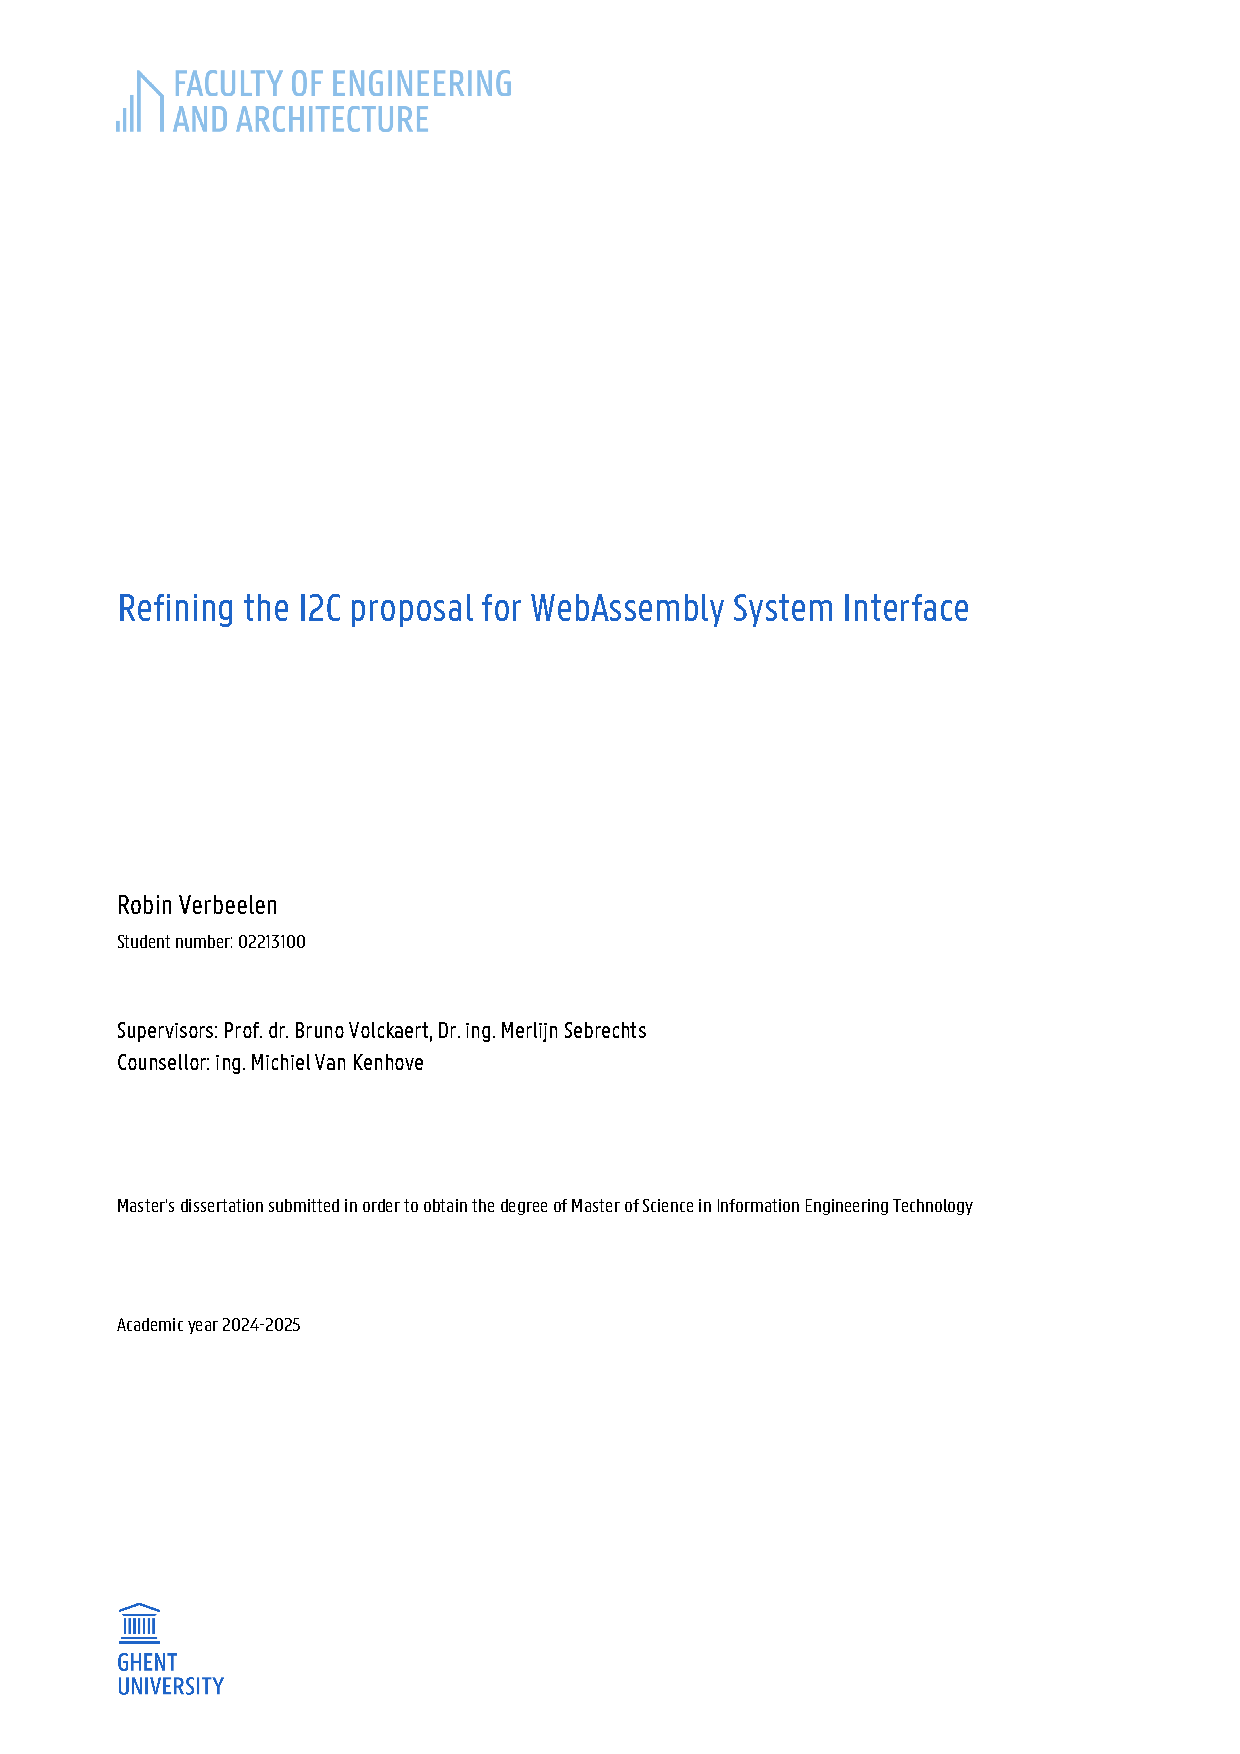
\includepdf{cover-sheet.pdf}

% Only add this Chapter if applicable
\chapter*{Statement of confidentiality}

Confidential up to and including dd/mm/yyyy

Important

This master’s dissertation contains confidential information and/or confidential research results proprietary to Ghent University or third parties. It is strictly forbidden to publish, cite or make public in any way this master’s dissertation or any part thereof without the express written permission of Ghent University. Under no circumstance may this master’s dissertation be communicated to or put at the disposal of third parties. Photocopying or duplicating it in any other way is strictly prohibited. Disregarding the confidential nature of this master’s dissertation may cause irremediable damage to Ghent University. The stipulations mentioned above are in force until the embargo date.
\chapter*{Acknowledgment}
\addcontentsline{toc}{chapter}{Acknowledgments}

I would like to express my sincere gratitude to all those who contributed to the successful completion of this master's thesis.

First and foremost, I extend my heartfelt thanks to my promotors, Prof. Dr. Bruno Volckaert and Dr. Merlijn Sebrechts, for placing their trust in me and providing the opportunity to participate in this research. Your confidence in my abilities has been invaluable throughout this journey.

Later in the year, Friedrich Vandenberghe, MSc in Industrial Engineering, joined our team as my predecessor on this thesis topic. Friedrich, your extensive experience with this research theme and your valuable contributions from the middle phase of my trajectory on have significantly enriched my work. Your insights and willingness to share your knowledge have been tremendously helpful.

I want to especially acknowledge Merlijn, Michiel, and Friedrich together again for always being available whenever I wanted to discuss results, share ideas, or seek advice. Your open-door policy and genuine interest in my progress have made this research journey both productive and enjoyable.

Finally, I would like to thank my girlfriend, friends, and parents for their unwavering support and genuine interest in my research. Your encouragement and curiosity about my work provided the extra motivation I needed to strive for excellent results. Your belief in me has been a constant source of strength throughout this challenging but rewarding experience.

This thesis would not have been possible without the collective support, guidance, and encouragement of all the individuals mentioned above. Thank you for making this journey memorable and successful.
\chapter*{Explanation regarding the master's thesis and the oral presentation}


This master's dissertation is part of an exam. Any comments formulated by the assessment committee during the oral presentation of the master's dissertation are not included in this text.

%%%%%%%%%%%%%%%%%%%%%%%%%%%%%%
%    Dutch version           %
%%%%%%%%%%%%%%%%%%%%%%%%%%%%%%
%
% \chapter*{Toelichting in verband met het masterproefwerk}
%
% Deze masterproef vormt een onderdeel van een examen. Eventuele opmerkingen die door de beoordelingscommissie tijdens de mondelinge uiteenzetting van de masterproef werden geformuleerd, werden niet verwerkt in deze tekst.
\chapter*{Abstract}
\chaptermark{Abstract}
\addcontentsline{toc}{chapter}{Abstract}  

This chapter should contain three things.

\begin{itemize}
    \item A copy of all the information on the title page of your master's thesis. This includes things like the name of your master's thesis and your advisors.
    \item A one-paragraph description of your master's thesis. This should be 15 to 20 lines long. This should include the context of your master's thesis, the problem statement of your master's thesis. The results of your master's thesis, and the evaluation of the work.
    \item Five keywords that describe the subject best.
\end{itemize}

The chapter should be one page at most.

% How to add the extended abstract:
%
% You should write the extended abstract as a separate overleaf project. Then compile it there, download the PDF, and upload it to this project.
%
% Use the "IEEE conference proceedings template" to create the extended abstract project. 
% https://www.overleaf.com/latex/templates/ieee-conference-template/grfzhhncsfqn
%
% Then download the final PDF, upload it to the root of this project, and point the statement below to the correct file.
\phantomsection
\addcontentsline{toc}{chapter}{Extended Abstract}
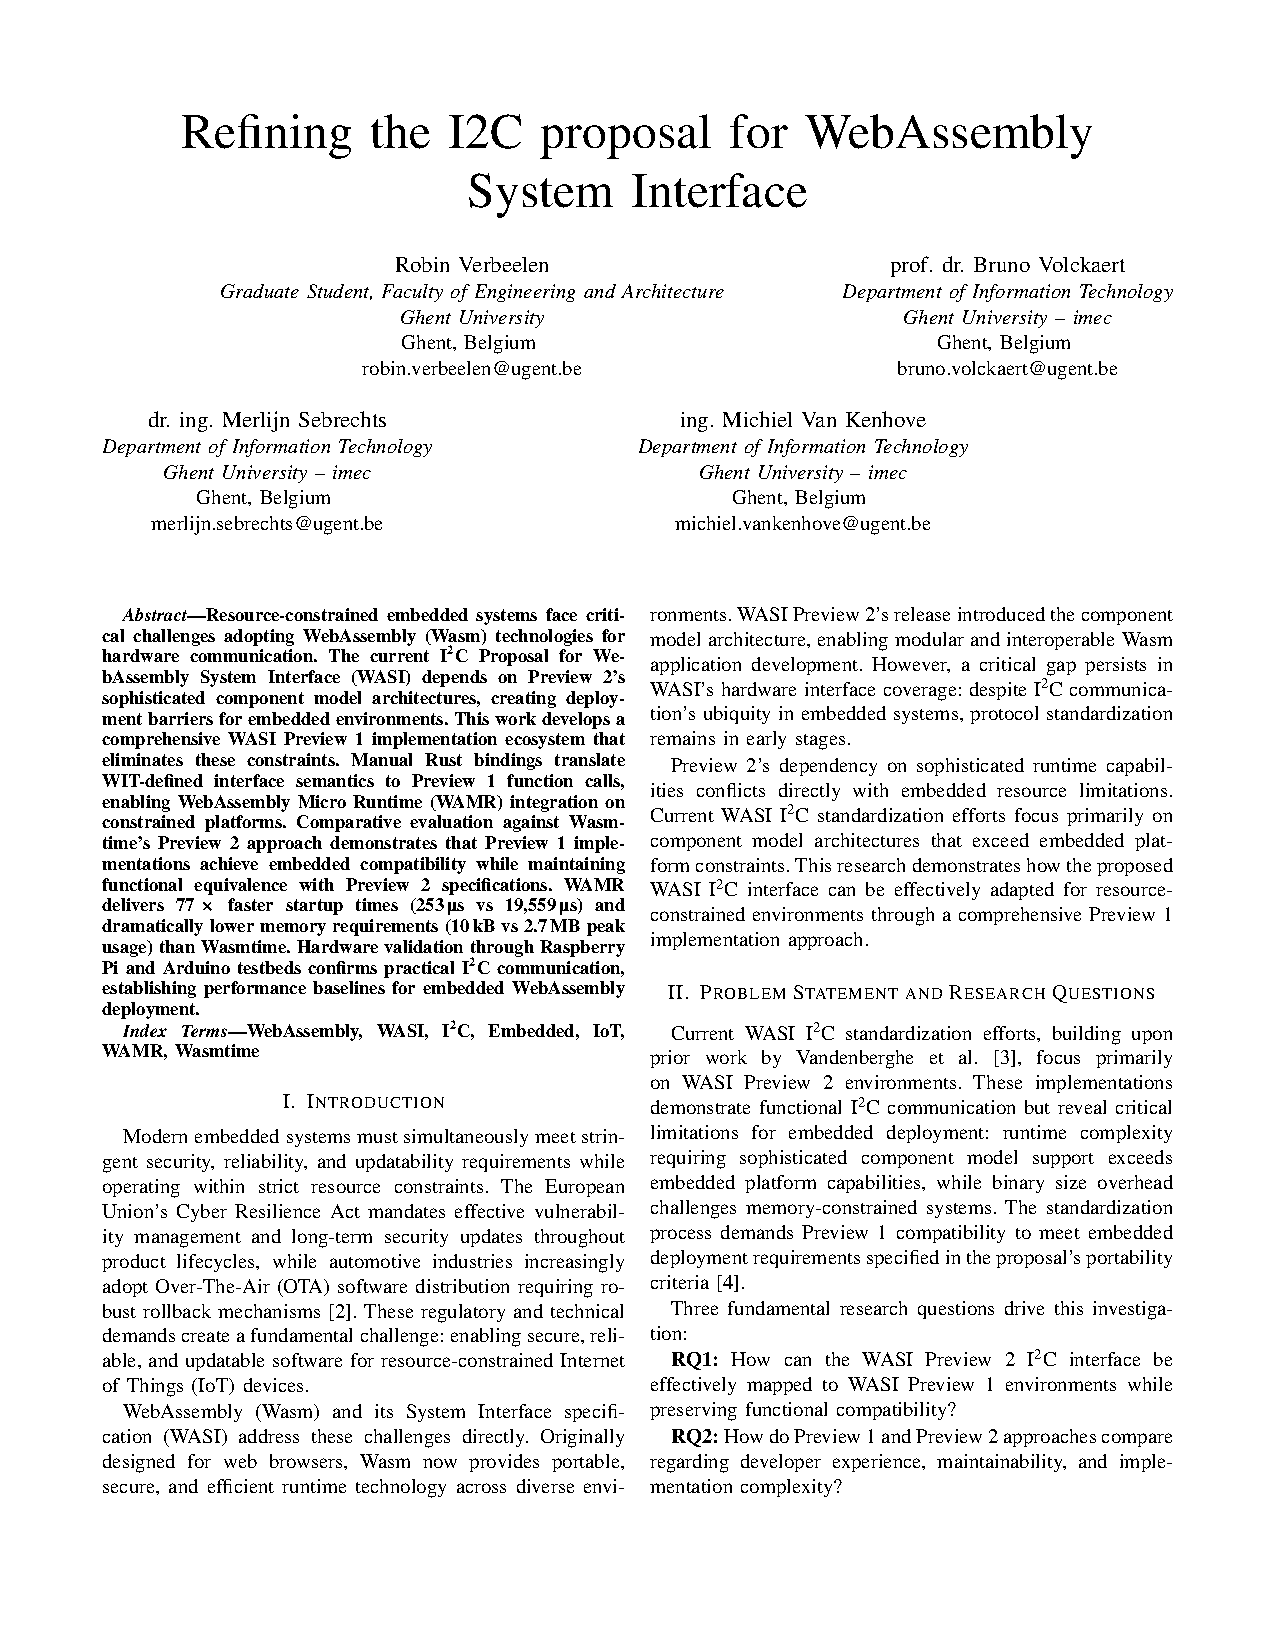
\includepdf[pages={-}]{extended-abstract.pdf}
\tableofcontents\newpage
\listoffigures\newpage
\listoftables\newpage
\printglossary[type=\acronymtype, title={List of Acronyms}]

\glsaddallunused[\acronymtype]                              % make sure all unused acronyms are in list

\setlist[description]{style=standard} % reset list settings back to default

\listoflistings\newpage

%
% Include the main chapters of the thesis below
% Note: it's best to avoid spaces in filenames as Latex might complain about them.
%
\mainmatter
\pagestyle{fancy} % Use header
\chapter{Introduction}
\label{chap:introduction}

Modern embedded systems face unprecedented challenges in balancing security, reliability, and updateability requirements while operating under strict resource constraints. The European Union's Cyber Resilience Act, enacted in March 2024, mandates that manufacturers ensure effective vulnerability management and provide security updates throughout a product's expected lifespan~\cite{eu_cyber_res_act}. Simultaneously, the automotive industry's rapid adoption of over-the-air (OTA) software distribution demands robust rollback capabilities when updates fail~\cite{automotive_ota}. These regulatory and industry pressures converge on a fundamental need: secure, reliable, and easily updatable software solutions that impose minimal overhead on resource-constrained Internet of Things (IoT) devices.

WebAssembly (Wasm) and its system interface specification, WASI (WebAssembly System Interface), represent a promising technological response to these challenges. Originally designed to execute binary code within web browsers, WebAssembly has evolved beyond its initial scope to enable portable, secure, and efficient code execution across diverse environments~\cite{wasm_spec}. WASI extends this capability by providing a standardized system interface that facilitates interaction with filesystems, network resources, and hardware peripherals while maintaining WebAssembly's core security guarantees through capability-based access control.

The emergence of WASI Preview 2, accompanied by the component model architecture, introduced sophisticated mechanisms for building interoperable WebAssembly libraries, applications, and environments. This component model utilizes \acrfull{wit} files to define interface contracts and enable automatic binding generation between components~\cite{wasi_p2}. However, a critical gap remains in WASI's hardware interface coverage: despite the ubiquity of Inter-Integrated Circuit (I2C) communication in embedded systems, the standardization of the WASI I2C interface is only in very early stages.

I2C represents one of the most widely deployed communication protocols in embedded systems, serving as the backbone for sensor communication, device configuration, and inter-chip data exchange in IoT applications~\cite{i2c_specification}. The protocol's simplicity, addressing efficiency, and multi-host capability have made it indispensable for embedded system designers. Yet, the early state of the WASI I2C interface creates a significant barrier to WebAssembly adoption in embedded environments where I2C communication is fundamental.






\section{Problem Statement and Research Context}
\label{sec:problem-statement}

Friedrich Vandenberghe's pioneering work established the foundation for WASI I2C standardization by advancing the proposal from its initial conceptual phase to Phase 2 of the official WASI standardization process~\cite{friedrich_thesis}. His investigation included WIT interface design and proof-of-concept implementations mainly targeting WASI Preview 2 environments. Friedrich's work demonstrated the technical feasibility of WASI I2C integration and provided performance characterizations for Wasmtime-based implementations.

However, Friedrich's implementation approach, while technically sound and aligned with the future direction of WebAssembly component model adoption, revealed a critical limitation for immediate embedded system deployment: dependency on WASI Preview 2 and the component model architecture. These technological requirements impose constraints that conflict with the resource limitations prevalent in embedded environments:

\begin{enumerate}
    \item \textbf{Runtime Complexity}: WASI Preview 2 implementations require sophisticated runtime environments with component model support, limiting compatibility with lightweight WebAssembly runtimes optimized for embedded deployment.
    
    \item \textbf{Binary Size Overhead}: More sophisticated runtimes combined with component model metadata and automatic binding generation introduce significant binary size increases, challenging deployment in memory-constrained embedded systems.
\end{enumerate}

These limitations represent a fundamental tension between the sophisticated developer experience provided by WASI Preview 2 and the resource constraints that define embedded system deployment scenarios. To advance the WASI I2C proposal towards Phase 3 standardization, a Preview 1-compatible implementation becomes essential. This allows for demonstrating compatibility with embedded device constraints.




\section{Research Questions}
\label{sec:research-questions}

This thesis addresses the following research questions, which collectively evaluate the feasibility of the WASI I2C proposal in resource-constrained embedded systems:

\begin{researchquestion}\label{rq1}
\textbf{How can the WASI Preview 2 I2C interface be effectively adapted for WASI Preview 1 environments while maintaining functional compatibility with the standardized Preview 2 specification?}
\end{researchquestion}

This question examines the technical challenges of manually implementing Preview 1 bindings that preserve the semantic richness of WIT-defined interfaces. It investigates type system adaptation strategies, error handling mechanism design, and resource management approaches that enable Preview 1 implementations to provide equivalent functionality to their Preview 2 counterparts.

\begin{researchquestion}\label{rq2}
\textbf{How do Preview 1 and Preview 2 approaches compare in terms of developer experience, maintainability, and implementation complexity?}
\end{researchquestion}

This question evaluates the development and maintenance trade-offs between manual binding implementation and automatic code generation.

\begin{researchquestion}\label{rq3}
\textbf{What are the performance implications of WASI Preview 2 compared to Preview 1 for embedded I2C applications?}
\end{researchquestion}

This question is about a quantitative comparison between WAMR (Preview 1) and Wasmtime (Preview 2) approaches across multiple performance dimensions. It examines startup latency, steady-state execution overhead, memory consumption patterns, and resource utilization efficiency to establish empirical foundations in Preview characteristics.




\section{Contributions and Thesis Structure}
\label{sec:contributions-structure}

This thesis makes several key contributions to the WASI I2C standardization effort and embedded WebAssembly deployment by developing a comprehensive Preview 1 implementation ecosystem that bridges the gap between resource-constrained embedded systems and modern WebAssembly standards.

\subsection{Research Contributions}
\label{subsec:research-contributions}

The primary contributions of this work include:

\begin{enumerate}
    \item \textbf{WASI Preview 1 I2C Bindings Library}: Development of a manual Rust bindings library that faithfully translates WIT-defined I2C interface semantics to Preview 1's function call mechanisms. This library preserves type safety, error handling capabilities, and maintains semantic compatibility with the official WASI I2C specification while operating within Preview 1 constraints.

    \item \textbf{Preview 1 Guest Implementation}: Creation of a WebAssembly Module targeting \sloppy\texttt{wasm32-wasip1} that demonstrates the usage of the Preview 1 bindings and functionality. The implementation emphasizes maintaining full functional compatibility with the Preview 2 Component version.
    
    \item \textbf{WAMR Integration}: Implementation of a complete host runtime based on WebAssembly Micro Runtime (WAMR) that provides I2C hardware access through careful integration between Rust's memory safety model and WAMR's C-based architecture. This contribution demonstrates practical embedded deployment strategies for WASI I2C applications.
    
    \item \textbf{Comparative Preview 2 Framework}: Development of a parallel WebAssembly Component and Wasmtime runtime implementation, enabling comprehensive comparison across different WebAssembly approaches for I2C communication.
    
    \item \textbf{Performance Evaluation Methodology}: Design and implementation of a rigorous benchmarking framework that measures startup latency, execution overhead, memory utilization, and resource efficiency across multiple runtime approaches, providing empirical foundations for embedded WebAssembly deployment decisions.
\end{enumerate}

\subsection{Thesis Organization}
\label{subsec:thesis-organization}

This thesis is structured to progressively address the research questions through a combination of background establishment, implementation development, and empirical evaluation:

\textbf{Chapter~\ref{chap:background}} establishes the technical foundation necessary for understanding the implementation challenges. It covers WebAssembly fundamentals, WASI architecture, the evolution from Preview 1 to Preview 2, WIT interface definition and binding generation mechanisms, WebAssembly runtime ecosystem characteristics, I2C protocol specifications, and the current state of the WASI I2C standardization proposal.

\textbf{Chapter~\ref{chap:implementation}} presents the complete development of the Preview 1 I2C ecosystem, detailing the manual bindings library design, WAMR host integration approaches, and the comparative Preview 2 implementation. This chapter directly addresses \textbf{\autoref{rq1}} by demonstrating how Preview 2 interface semantics can be effectively adapted for Preview 1 environments, and contributes to \textbf{\autoref{rq2}} by examining the implementation complexity and developer experience trade-offs between manual and automatic binding approaches.

\textbf{Chapter~\ref{chap:eval}} details the experimental methodology and presents comprehensive performance evaluation results. Through controlled hardware experiments using Raspberry Pi and Arduino platforms, this chapter provides a statistical analysis of timing characteristics, memory utilization patterns, and resource efficiency comparisons. The empirical findings directly address \textbf{\autoref{rq3}} by quantifying the performance implications of different WebAssembly runtime approaches for embedded I2C applications.

\textbf{Chapter~\ref{chap:conclusion}} synthesizes the experimental findings and implementation insights to provide definitive answers to all research questions. It examines the broader implications for embedded WebAssembly deployment, discusses the limitations of the current approach, and outlines the impact on WASI I2C standardization efforts.

\textbf{Chapter~\ref{chap:future-work}} identifies promising research directions that extend this work toward production-ready deployment scenarios.

\textbf{Chapter~\ref{chap:ethics}} briefly examines the ethical considerations surrounding WebAssembly for I2C standardization and its potential impact on technology accessibility and environmental sustainability.

This investigation provides practical guidance for embedded system developers considering WebAssembly adoption while directly supporting the WASI I2C standardization effort through the demonstration of embedded system compatibility. The findings inform ongoing standardization discussions regarding the balance between sophisticated developer experiences and resource-constrained deployment requirements, ultimately contributing to the advancement of WebAssembly in embedded computing environments.
\chapter{Background}
\label{chap:background}

This chapter provides the essential background knowledge required to understand the contributions of this research, with particular attention to \acrshort{wasm}, \acrshort{wasi}, the \acrshort{i2c} communication protocol, and relevant runtime environments.

\section{WebAssembly}
\label{sec:webassembly}

\subsection{Overview and Motivation}
\label{subsec:wasm-overview}

\acrfull{wasm} is a binary instruction format for a stack-based virtual machine designed as a portable compilation target for programming languages~\cite{rossberg2018webassembly, wasm_specs, w3c2022wasm2}. It was originally developed to enable near-native execution performance of code in web browsers. \acrshort{wasm} emerged from a collaborative effort by engineers from the four major browser vendors (Mozilla, Google, Microsoft, and Apple) to address the performance limitations of JavaScript while preserving the security and portability characteristics essential for web execution.

However, developers quickly recognized that \acrshort{wasm}'s unique combination of performance, security, and portability extended far beyond browser environments. Its sandboxed execution model enables near-native performance across diverse hardware architectures while maintaining strict security guarantees. These properties proved particularly valuable for embedded systems and \acrshort{iot} devices, where code must execute safely on resource-constrained hardware.

The introduction of the \acrfull{wasi} marked a pivotal transition from web-centric to general-purpose computing. \acrshort{wasi} provides standardized \acrshort{api} for functionalities such as filesystem access, clocks, and proposals for networking and system interactions, enabling \acrshort{wasm} modules to operate independently of browsers. The capability-based security model inherent in \acrshort{wasi} further addresses critical concerns in embedded deployments, where unauthorized access to hardware peripherals could compromise device functionality or user safety.

This evolution has proven timely. Critical infrastructure software and consumer products --- ranging from baby monitors to smartwatches --- have created unprecedented demand for technology that is secure, reliable, and easily updatable while requiring minimal overhead. Regulatory frameworks such as the European Parliament's Cyber Resilience Act~\cite{eu_cyber_res_act} further emphasize this need, as they oblige manufacturers to handle vulnerabilities effectively during support periods and to provide security updates throughout a product's expected lifespan. \acrshort{wasm}'s ability to deliver secure, cross-platform execution with straightforward update mechanisms positions it as a promising solution for these emerging requirements in safety-critical and resource-constrained environments.

\subsection{The WebAssembly Ecosystem}
\label{subsec:wasm-ecosystem}

The \acrshort{wasm} ecosystem comprises several components that enable the development, compilation, and execution of \acrshort{wasm} applications. These components include:

\textbf{Compilation Toolchains:} Several compilers can target \acrshort{wasm}, including Emscripten for C/C++~\cite{emscripten_git}, the Rust compiler with Tier~2 support~\cite{rust_wasm_target}, \texttt{wasi-sdk}~\cite{wasisdk}, and specialized tools such as AssemblyScript~\cite{assemblyscript_git}. These toolchains translate high-level languages into \acrshort{wasm} bytecode while managing language-specific runtime requirements.

\textbf{Runtime Environments:} \acrshort{wasm} can execute in browsers through built-in JavaScript engines such as V8~\cite{v8_wasm}. In addition, standalone runtimes like \acrshort{wamr}, Wasmtime, and Wasmer support server-side and embedded applications. These runtimes provide the execution environment and implement the \acrshort{wasm} specification~\cite{wasm_specs}.

\textbf{Development Tools:} The ecosystem includes debugging tools, profilers, and analysis frameworks that support \acrshort{wasm} development. Utilities such as \texttt{wasm-tools}~\cite{wasm_tools_git} and WABT (WebAssembly Binary Toolkit)~\cite{wabt_git} enable tasks like validation, disassembly, and binary inspection of \acrshort{wasm} modules.

\textbf{Standards and Governance:} \acrshort{wasm} development follows the W3C standardization process. Its evolution is coordinated through the WebAssembly Community Group and the W3C WebAssembly Working Group, ensuring that the technology advances in a consensus-driven and vendor-neutral manner.

\section{The WebAssembly System Interface}
\label{sec:wasi}

\subsection{Fundamentals}
\label{subsec:wasi-fundamentals}

\acrfull{wasi} represents a crucial evolution in \acrshort{wasm}'s capabilities, extending the platform beyond browser environments to enable execution in servers, edge devices, and embedded systems~\cite{wasi_mozilla_blog}. \acrshort{wasi} functions as a system interface for a conceptual operating system, providing a standardized way for \acrshort{wasm} modules to interact with system resources while preserving the security and portability characteristics that define the technology.

\acrshort{wasi} emerged from the need for \acrshort{wasm} programs outside the browser to interact with the underlying system. \acrshort{wasi} aims to provide this by defining a modular set of \acrshort{api}s --- through proposals --- that enable access to filesystems, networking, cryptographic functions, hardware interfaces, and more~\cite{wasi_proposals}.

The design philosophy of \acrshort{wasi} centers on capability-based security, where access to system resources is mediated through explicitly granted permissions rather than implicit, ambient authority (such as unrestricted filesystem access). This ensures that \acrshort{wasm} modules can only interact with resources explicitly provided by the host environment, thereby maintaining strong isolation and security even in server and embedded contexts.

\subsection{WASI Preview 1}
\label{subsec:wasi-preview1}
Preview 1 was the first stabilized release of \acrfull{wasi}, focused on providing fundamental system interaction capabilities. It employed WITX~\cite{witx_docs} as its \acrfull{idl}~\cite{idl}, an experimental language designed specifically for expressing \acrshort{wasi} \acrshort{api}s. WITX, based on S-expressions~\cite{sexpressions} and inspired by the WebAssembly Text (WAT) format~\cite{wat}, followed a function-oriented model closely resembling traditional system call interfaces. Although effective, WITX has since been deprecated in favor of the more flexible \acrshort{wit} format.

The design of Preview 1 drew heavily from POSIX conventions, implementing familiar concepts such as file descriptors, path-based file operations, and process-centric resource management. Its \acrshort{api} included essential system operations such as file handling (open, close, read, write), clocks and timers, random number generation, environment variable access, and command-line argument parsing.

Preview 1 saw widespread adoption thanks to its stability and practical utility. However, the WITX-based design revealed several fundamental limitations, including limited expressiveness and lack of modularity. These shortcomings motivated the \acrshort{wasi} Subgroup to transition toward the more sophisticated \acrshort{wit} format and the Preview 2 architecture:

\textbf{Limited Language Support:} WITX primarily targeted C-like languages and lacked the expressiveness to support a broader range of programming paradigms. Its design assumptions made it difficult to generate idiomatic bindings for languages with richer memory models, type systems, or runtime features.


\textbf{Restricted Type Expressiveness:} WITX offered only basic type safety, with limited support for strings and arrays, and no way to model complex return values. Functions typically returned success or failure via the \texttt{expected} construct, while actual data was passed through pointer parameters. This C-style pattern complicated memory management and hindered the design of clean, language-agnostic \acrshort{api}s.

\textbf{Monolithic Structure:} Preview 1 exposed a relatively monolithic API surface that was difficult to extend, compose, or virtualize. This lack of modularity prevented fine-grained capability management and made it impossible to define specialized subsets of the \acrshort{api} for targeted use cases.

These shortcomings led to the introduction of the more powerful \acrshort{wit} format and the component model in \acrshort{wasi} Preview 2. With this transition, WITX is now considered a legacy format and is no longer actively maintained.

\subsection{WASI Preview 2 and the Component Model}
\label{subsec:wasi-preview2}

Preview 2 constitutes a comprehensive redesign of \acrshort{wasi}. Whereas Preview 1 suffered from limited type expressiveness, poor language support, and a monolithic \acrshort{api} surface, Preview 2 introduces a modular architecture with advanced capabilities for component composition, virtualization, and language interoperability.

\textbf{Component Model:} A central innovation of Preview 2 is the Component Model~\cite{wasi_component_model}, which enables the composition of \acrshort{wasm} modules through well-defined interfaces. Components can both export and import functionality via standardized \acrshort{wit}-based descriptions, facilitating language interoperability and supporting complex application architectures with multiple interacting components.

\textbf{Resource-Based Design:} Unlike Preview 1’s function-oriented \acrshort{api}s, Preview 2 adopts a resource-based design in which system entities (e.g., files, sockets, or \acrshort{i2c} devices) are modeled as first-class resources with associated methods. This model improves encapsulation, enables automatic resource management, strengthens type safety, and aligns with capability-based security principles.

\textbf{WIT Interface Definition:} Preview 2 adopts the \acrshort{wit} format for defining interfaces. \acrshort{wit} supports complex data structures, resource types, and interface composition. Tooling such as \sloppy\texttt{wit-bindgen} can automatically generate idiomatic bindings for multiple programming languages, thereby improving developer productivity and interoperability.

\textbf{Capability-Based Security Enhancement:} The component model extends \acrshort{wasi}'s capability-based security by introducing fine-grained control over resource access and enabling explicit capability delegation between components. This design supports advanced scenarios such as capability attenuation, resource multiplexing, and policy enforcement—features particularly relevant in multi-tenant or embedded \acrshort{iot} environments.

\subsection{Differences and Trade-offs between Preview 1 and Preview 2}
\label{subsec:preview-differences}
The transition from Preview 1 to Preview 2 introduces significant differences and trade-offs. While Preview 2 improves expressiveness, modularity, and language interoperability, these advances also affect runtime implementation complexity, performance characteristics, and deployment scenarios:

\textbf{Memory Architecture:} Preview 1 and Preview 2 adopt fundamentally different approaches to memory management and inter-module communication. Preview 1 follows a shared-memory model, where modules exchange data through exported linear memory and raw pointer manipulation. \acrshort{api}s mutate caller-provided buffers directly, which requires modules to share a memory space for data exchange. In contrast, Preview 2 implements a strict shared-nothing architecture: each component instance encapsulates its own memory, tables, globals, and functions. Components interact exclusively through import/export boundaries defined in \acrshort{wit}, ensuring safer isolation, better type safety, and improved language interoperability.

\textbf{Implementation Complexity:} The component model in Preview 2 introduces significant complexity for runtime implementers. Supporting component instantiation, interface resolution, resource management, and the shared-nothing linking model requires a more sophisticated infrastructure than Preview 1’s relatively simple function dispatch with shared memory access. Furthermore, the transition from raw pointer-based interfaces to high-level type abstractions necessitates additional translation layers and the full implementation of the Canonical \acrfull{abi}~\cite{abi, cabi}, which may increase runtime overhead.

\textbf{Development Experience:} For developers, Preview 2 offers a significantly enhanced experience through automatic binding generation, improved type safety, and stronger tooling support. By eliminating raw pointer manipulation, it mitigates common security vulnerabilities such as buffer overflows and out-of-bounds memory access.

\textbf{Performance Implications:} The contrasting architectures of Preview 1 and Preview 2 lead to distinct performance characteristics. Preview 1’s shared-memory model allows efficient data exchange through direct pointer manipulation and zero-copy operations within a common address space. By contrast, Preview 2 employs the Canonical \acrshort{abi}, which specifies how high-level component types are represented as low-level \acrshort{wasm} types. Although the specification describes lifting and lowering operations that may seem to introduce intermediate copies, practical implementations often fuse these into efficient direct transfers between component memory spaces. The Canonical \acrshort{abi} is further optimized to avoid redundant copying, especially for immutable data structures that can be shared safely. Nonetheless, actual performance depends strongly on the chosen data types, mutability requirements, and component design. In addition, Preview 2’s resource-based model and component instantiation overhead can increase startup latency compared to Preview 1’s direct function-call approach, an effect particularly relevant in constrained environments and short-lived workloads.

\section{Binding Generation}
\label{sec:wit-binding}

\subsection{Binding Generation Process}
\label{subsec:binding-generation}

Binding generation transforms \acrshort{wit} interface definitions into language-specific code that enables type-safe access to WebAssembly component functionality. This process typically involves multiple stages that ensure correct data marshaling (encoding/serialization and decoding/deserialization) across component boundaries while preserving the semantic properties defined in the \acrshort{wit} interface. In practice, tools such as \texttt{wit-bindgen} automate this workflow for a wide range of programming languages~\cite{wit_bindgen_git}.

\textbf{Interface Analysis:} The binding generator parses \acrshort{wit} definitions to extract type information, resource dependencies, and interface relationships. This analysis phase validates the interface definition and constructs an intermediate representation suitable for code generation.

\textbf{Type Mapping:} In the second stage, \acrshort{wit} types are mapped to idiomatic representations in the target language. For example, a \texttt{u32} in \acrshort{wit} may be mapped to \texttt{u32} in Rust, \texttt{int} in C, or \texttt{number} in JavaScript. The goal is to balance semantic fidelity with a natural developer experience in the chosen language.

\textbf{Marshaling Code Generation:} In this stage, the generator produces code that converts between language-native types and their Canonical \acrshort{abi} representations for inter-component communication. This marshaling is bidirectional, ensuring that both host-to-guest and guest-to-host calls are correctly translated. It includes handling of complex data structures, resource handles, and error propagation across component boundaries.

\textbf{Resource Management Integration:} Finally, the generator aligns resource lifecycle management with the conventions of the target language. In garbage-collected languages such as Java or Python, this involves integrating with the runtime’s memory management system. In contrast, languages like Rust rely on explicit ownership and \acrfull{raii} semantics, where the generator ensures that imported and exported resources are correctly created, transferred, and dropped at well-defined points in the program’s execution.

Popular binding generation tools include:

\begin{itemize}
    \item \textbf{wit-bindgen:} The primary reference implementation that generates idiomatic bindings for multiple target languages including Rust, C, JavaScript, and Python~\cite{wit_bindgen_git}. It is widely adopted in the component model ecosystem.
    \item \textbf{Wasmtime bindgen macro:} A Rust-specific integration that provides compile-time binding generation directly within the Wasmtime runtime, enabling seamless use of \acrshort{wit}-defined interfaces in Rust projects~\cite{wasmtime_bindgen_docs}.
    \item \textbf{jco:} A JavaScript-focused tool that simplifies component development and execution in Node.js and browser environments~\cite{jco_docs}.
    \item \textbf{wasm-tools:} A broader toolkit maintained by the Bytecode Alliance that provides validation, parsing, and transformation utilities, including support for \acrshort{wit} integration~\cite{wasm_tools_git}.
\end{itemize}

\subsection{Binding Generation vs Manual Implementation}
\label{subsec:binding-comparison}

The decision between relying on automatic binding generation and opting for manual interface implementation introduces trade-offs across multiple dimensions, including development efficiency, runtime performance, and overall implementation complexity. While automatic tools provide rapid development and reduce the likelihood of errors, manual implementations allow for fine-grained control at the cost of increased effort and potential maintenance overhead.

\begin{table}[H]
    \centering
    \begin{tabular}{|C{2.1cm}|C{6cm}|C{6cm}|}
    \hline
            & \textbf{Automatic Binding Generation} & \textbf{Manual Implementation} \\
    \hline
    \textbf{Development Efficiency} & Eliminates manual interface interpretation, prone to errors. Enables rapid prototyping and higher reliability. & Requires handwritten marshaling logic and careful error handling. Higher initial effort and increased chance of bugs. \\
    \hline
    \textbf{Type Safety} & Provides compile-time type safety guarantees. & Relies on developer discipline to ensure correct type conversions. \\
    \hline
    \textbf{Performance} & May include some abstraction overhead, but benefits from systematic optimization in the generator. & Can be optimized for specific use cases and low-level constraints, potentially achieving lower overhead. \\
    \hline
    \textbf{Maintenance} & Automatically adapts to interface changes when regenerating bindings. & Requires manual updates whenever the interface evolves. Long-term maintenance burden. \\
    \hline
    \textbf{Runtime Compatibility} & May require sophisticated runtime capabilities (e.g., Preview 2 features) & Can be tailored to specific runtimes, \acrshort{wasi} versions or environments, offering maximal flexibility. \\
    \hline
    \end{tabular}
    \caption{Comparison between automatic binding generation and manual implementation approaches.}
    \label{tab:binding-vs-manual}
\end{table}












\section{WebAssembly Runtimes}
\label{sec:wasm-runtimes}

\subsection{Runtime Architecture and Design Principles}
\label{subsec:runtime-architecture}

WebAssembly runtimes provide the execution environment for \acrshort{wasm} modules and components, offering infrastructure for loading, validating, compiling, and executing code. Architectural decisions differ between runtimes and strongly influence performance, resource usage, and deployment suitability~\cite{wasm_features_support}.

The fundamental components of a typical WebAssembly runtime include:

\begin{itemize}
    \item \textbf{Module Loader and Validator:} Parses the WebAssembly binary format, validates module structure and type safety, and ensures compliance with WebAssembly’s security guarantees.
    \item \textbf{Execution Engine:} Implements WebAssembly’s execution semantics through interpretation, \acrfull{jit} compilation, or \acrfull{aot} compilation. The chosen strategy affects startup latency, memory footprint, and steady-state performance.
    \item \textbf{Memory Management:} Manages WebAssembly’s linear memory model, including allocation, growth, and bounds checking. Linear memory differs from conventional memory layouts by exposing a single contiguous address space to the guest.
    \item \textbf{Host Interface:} Provides controlled access to system resources via \acrshort{wasi} or custom host functions, enabling I/O and integration with native libraries.
    \item \textbf{Security Sandbox:} Enforces isolation between the WebAssembly module and the host, preventing out-of-bounds memory access and restricting system calls to a well-defined capability model.
\end{itemize}

\subsection{Wasmtime}
\label{subsec:wasmtime}

Wasmtime is a production-ready runtime maintained by the Bytecode Alliance and is widely regarded as the reference implementation for \acrshort{wasi} and the WebAssembly Component Model~\cite{wasmtime_project}. Its architecture emphasizes standards compliance, security, and developer experience, making it the primary choice for developing \acrshort{wasi} Preview~2 applications.

\textbf{Cranelift Code Generation:} Wasmtime uses Cranelift, a compiler backend designed for security and fast compilation speed while providing competitive runtime performance~\cite{cranelift}. Cranelift supports both \acrshort{jit} compilation for dynamic workloads and \acrshort{aot} compilation for deployment scenarios requiring lower startup latency.

\textbf{Language Integration:} Wasmtime provides high-quality libraries for multiple host languages, including Rust, C/C++, Python, and JavaScript. This broad ecosystem integration facilitates embedding Wasmtime into diverse application environments and frameworks.

\subsection{WebAssembly Micro Runtime}
\label{subsec:wamr}

\acrfull{wamr} is a lightweight and portable WebAssembly runtime specifically designed for embedded devices, \acrshort{iot} applications, and resource-constrained environments~\cite{wamr_project, wamr_project2}. Its architecture prioritizes minimal resource usage, fast startup, and broad platform compatibility, making it suitable for deployment scenarios where memory and processing resources are limited.

\textbf{Lightweight Design Philosophy:} WAMR minimizes memory footprint and startup overhead, which are essential for embedded deployments. This distinguishes it from general-purpose runtimes such as Wasmtime.

\textbf{Execution Engine Options:} WAMR supports multiple execution strategies, including interpretation, Classic \acrshort{jit}, Fast \acrshort{jit}, and \acrshort{aot} compilation. The execution mode can be configured to match the performance and resource constraints of the target device. For example, \acrshort{aot} compilation is often preferred for microcontrollers, where runtime compilation would be impractical.

\textbf{Platform Portability:} WAMR runs on a wide range of platforms, including popular microcontroller architectures (e.g., ARM Cortex-M, RISC-V), real-time operating systems such as Zephyr and FreeRTOS, and constrained Linux environments. This versatility enables adoption in diverse embedded use cases.

\textbf{WASI Preview 1 Focus:} WAMR primarily supports \acrshort{wasi} Preview~1, which aligns with the stability and simplicity requirements of embedded applications. While Preview~2 support is under consideration, Preview~1 remains the main interface for production deployments. This Preview~1 focus is a key reason for using WAMR in this research, since it necessitates the development of custom bindings for the \acrshort{i2c} interface.


\section{I2C Protocol and Embedded Systems}
\label{sec:i2c-embedded}

\subsection{Protocol Fundamentals}
\label{subsec:i2c-fundamentals}

The \acrfull{i2c} protocol is a multi-controller\footnote{Following the updated terminology "controller/target" instead of "master/slave" to align with the MIPI I3C specification and NXP's Inclusive Language Project~\cite{i2c_specification}.}, multi-target serial communication bus widely used in embedded systems for connecting microcontrollers with peripheral devices~\cite{i2c_specification}. Developed by Philips Semiconductor (now part of NXP Semiconductors) in the early 1980s, \acrshort{i2c} has become a fundamental communication protocol in \acrshort{iot} ecosystems, sensor networks, and embedded control systems. Although the specification allows for multiple controllers, most practical implementations rely on a single controller with multiple targets.

The protocol operates over two bidirectional signal lines: the \textbf{Serial Data Line (SDA)}, which carries the data being transmitted, and the \textbf{Serial Clock Line (SCL)}, which provides the clock signal controlled by the initiating controller. Both lines are implemented as open-drain outputs with pull-up resistors, enabling multiple devices to share the same bus safely.

\subsection{I2C Communication Mechanisms}
\label{subsec:i2c-communication}

\textbf{Device Addressing:} Each target device on the \acrshort{i2c} bus has a unique address, typically 7 bits in length. Although a 10-bit addressing mode exists, it is less common in practice.

\textbf{START, Repeated START, and STOP Conditions:} Communication sessions begin with a START condition and end with a STOP condition, both defined by transitions on SDA while SCL is high. A repeated START allows a controller to retain bus control without releasing it, which is frequently used in read transactions.

\textbf{Acknowledgment Mechanism:} Each transmitted byte must be acknowledged (ACK) by the receiving device. A missing acknowledgment (NACK) indicates either that no device responded at the specified address, or that the controller has signaled the end of the transfer.





\textbf{Multi-Controller Support:} The \acrshort{i2c} protocol includes arbitration mechanisms allowing multiple controllers to coexist on the same bus. Arbitration ensures that when two controllers attempt simultaneous communication, only one retains control without corrupting data. In practice, however, most \acrshort{i2c} systems are deployed with a single controller~\cite{i2c_specification}.

\subsection{Hardware Abstraction Layers}
\label{subsec:hal-embedded}

\acrfull{hal}s provide portable interfaces to access hardware peripherals, abstracting device-specific details behind generic \acrshort{api}s. This decoupling allows driver code to operate across different microcontroller families and platforms~\cite{hal}.  

In the Rust ecosystem, the \texttt{embedded-hal} crate~\cite{embedded_hal_crate} has become the de facto standard, defining traits for common peripherals such as \acrshort{i2c}, SPI, GPIO, and UART. Numerous driver crates build on these traits, ensuring cross-platform portability. Platform-specific implementations include \texttt{linux-embedded-hal}~\cite{linux_embedded_hal_crate} for Linux systems and other crates targeting Raspberry Pi~\cite{rppal_crate} or STM32 microcontrollers~\cite{stm_hal_crate}.

\section{WASI I2C Standardization Proposal}
\label{sec:wasi-i2c-proposal}

\subsection{Standardization Process and Current Status}
\label{subsec:i2c-standardization-process}

The \acrshort{wasi} \acrshort{i2c} proposal is part of the ongoing effort to standardize hardware communication interfaces within the \acrshort{wasi} specification~\cite{wasi_i2c_proposal}. Standardization in the \acrshort{wasi} subgroup follows a structured process with multiple phases: conceptual start (Phase 0), exploratory design (Phase 1), prototyping and specification drafting (Phase 2), implementation and integration (Phase 3), and final standardization (Phase 4-5).  

The \acrshort{i2c} proposal is currently in Phase~2, focusing on prototyping, implementation feasibility, and iterative design refinement. To advance to Phase~3, it must demonstrate comprehensive test coverage, resolve open design questions, and show multiple independent implementations.

\subsection{Proposal Architecture and Design}
\label{subsec:i2c-proposal-design}

The \acrshort{wasi} \acrshort{i2c} proposal~\cite{wasi_i2c_proposal} defines an interface inspired by the design principles of \texttt{embedded-hal} v1~\cite{hal}, while adapting them to the \acrshort{wasm} Component Model's resource-based architecture. The proposal consists of three primary \acrshort{wit} files that together form a modular and composable interface design:

\textbf{Core Interface Components:}
\begin{itemize}
    \item \textbf{i2c.wit:} Defines the primary \acrshort{i2c} communication interface, including transaction operations, read/write methods, and error handling.
    \item \textbf{delay.wit:} Provides timing and delay functionality required for \acrshort{i2c} protocol compliance and device timing requirements.
    \item \textbf{world.wit:} Specifies the complete interface surface that components must either implement or import.
\end{itemize}

\textbf{Resource-Based Design:} The proposal implements \acrshort{i2c} controllers as first-class resources in the Component Model, enabling proper lifetime management and capability-based security. This design ensures that \acrshort{i2c} access is mediated through explicit capability grants rather than ambient authority.

\textbf{Error Handling Strategy:} The interface defines comprehensive error types that cover common \acrshort{i2c} failure modes such as bus errors, arbitration loss, and acknowledgment failures. In addition, device-specific conditions (e.g., a non-existent register address being accessed or a timeout during EEPROM operations) are modeled explicitly. This detailed error modeling enables robust error recovery and diagnostic capabilities.

\textbf{Operation Support:} The interface supports both simple read/write operations and complex transaction sequences, enabling efficient communication patterns required by various \acrshort{i2c} devices and protocols.

\subsection{Portability Criteria}
\label{subsec:i2c-portability}

To be viable as a standardized interface, the \acrshort{wasi} \acrshort{i2c} proposal must satisfy portability criteria that demonstrate applicability across diverse implementation environments and hardware platforms. Table~\ref{tab:portability_criteria} summarizes the minimal platforms selected to validate cross-architecture support.

\begin{table}[H]
    \centering
    \captionsetup{justification=centering}
    \caption{Minimal hardware platforms selected as portability criteria for advancing the I\textsuperscript{2}C proposal}
    \label{tab:portability_criteria}
    \begin{tabular}{lll}
        \toprule
        \textbf{Platform} & \textbf{Architecture} & \textbf{Reference Hardware} \\
        \midrule
        Linux & ARM & Raspberry Pi 3 Model B \\
        RTOS (NuttX or Zephyr) & RISC-V & ESP32-C3 \\
        RTOS (Zephyr or FreeRTOS) & ARM32 & Nucleo F412ZG \\
        \bottomrule
    \end{tabular}
\end{table}

Table~\ref{tab:portability_criteria_specs} provides detailed hardware specifications of the selected platforms. The limited RAM and Flash memory of the Nucleo board pose a particular challenge for implementing the full proposal.

\begin{table}[H]
    \centering
    \caption{Hardware specifications of the platforms used in the portability criteria}
    \label{tab:portability_criteria_specs}
    \begin{tabular}{lL{4cm}L{2cm}L{3cm}L{1.5cm}}
        \toprule
        \textbf{Platform} & \textbf{Processor} & \textbf{RAM} & \textbf{Storage/Flash} & \textbf{GPIO} \\
        \midrule
        Raspberry Pi 3 Model B & 
        Broadcom BCM2837 ARM Cortex-A53 64-bit quad-core @ 1.2 GHz & 
        1 GB LPDDR2 & 
        microSD card & 
        40-pin header \\
        \hline
        ESP32-C3 & 
        Single-core 32-bit RISC-V (RV32IMC) @ 160 MHz & 
        400 KB SRAM & 
        384 KB ROM + 2--8 MB external flash & 
        22 pins \\
        \hline
        Nucleo F412ZG & 
        ARM Cortex-M4F with FPU @ 100 MHz & 
        256 KB SRAM & 
        1 MB Flash memory & 
        114 I/O pins\footnote{Not all GPIO pins are available through the Nucleo board headers.} \\
        \bottomrule
    \end{tabular}
\end{table}



\subsection{Integration with Embedded-HAL Principles}
\label{subsec:i2c-embedded-hal-integration}

The \acrshort{wasi} \acrshort{i2c} proposal deliberately aligns with the design principles of the \acrshort{hal} project~\cite{hal}, ensuring compatibility with the existing Rust embedded ecosystem and leveraging proven interface abstractions. This alignment facilitates adoption by embedded developers and enables reuse of existing device driver implementations.

\textbf{Trait Compatibility:} The \acrshort{wit}-based interface design closely maps to the \texttt{embedded-hal} \acrshort{i2c} traits. This enables straightforward adaptation of existing drivers to the \acrshort{wasi} \acrshort{i2c} interface through thin wrapper implementations, minimizing the need for substantial code changes.

\textbf{Error Model Alignment:} The proposal’s error handling strategy follows the conventions established in \texttt{embedded-hal}, while extending error categories to support richer diagnostics in a \acrshort{wasm} environment. For example, errors can include additional context such as bus arbitration failures or timeouts that may not be captured by traditional embedded traits.

\textbf{Operation Semantics:} Transaction semantics, addressing models, and timing requirements are defined in close correspondence with \texttt{embedded-hal} expectations. In particular, the use of the dedicated \texttt{delay.wit} interface mirrors the \texttt{DelayUs} and \texttt{DelayMs} traits, ensuring that timing-sensitive communication can be modeled consistently across both embedded and WebAssembly environments.
\chapter{Implementation}
\label{chap:implementation}

This chapter presents the implementation details of a WASI Preview 1 I2C interface designed specifically for \acrshort{wamr}, addressing the critical requirement for embedded device support in the WASI I2C standardization proposal. Building upon Friedrich's foundational work~\cite{friedrich_paper}~\cite{friedrich_impl}, this implementation establishes a comprehensive Preview 1 setup that enables resource-constrained embedded systems to participate in the I2C standardization effort.

The implementation serves as an exploration of how the WASI I2C interface could be adapted for Preview 1 environments, providing essential groundwork for the proposal's progression to the next standardization phase, which requires demonstrated compatibility with embedded device constraints.

\section{System Overview \& Architecture}
\label{sec:system-overview}

\subsection{Implementation Context and Scope}

The development effort encompasses five core implementations that collectively demonstrate Preview 1 I2C interface feasibility:

\begin{minted}{text}
    wasip1-i2c-lib/          // Manual Preview 1 bindings library
    wasip1-i2c-guest/        // Core WASM module (target: wasm32-wasip1)
    wasip2-i2c-guest/        // WASM component (target: wasm32-wasip2)
    wamr_impl/               // WAMR host runtime implementation
    wasmtime_impl/           // Wasmtime host runtime implementation
\end{minted}

\begin{figure}[h]
	\centering
	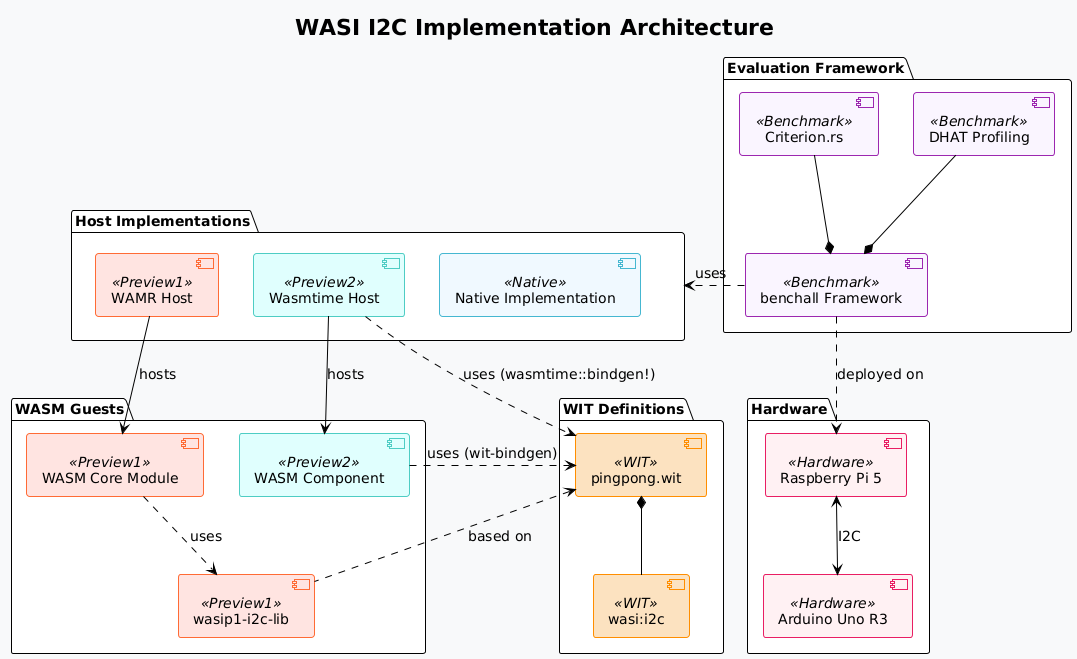
\includegraphics[width=\textwidth]{images/project schema.png}
	\caption{Overview of the project structure, showcasing the structure and interaction between different components}
	\label{fig:project_schema}
\end{figure}

All implementations in this ecosystem, including the Preview 2 component and Wasmtime host, represent original contributions developed specifically for this research. The system design enables direct comparison between Preview 1 and Preview 2 approaches while maintaining functional equivalence in I2C communication capabilities.

\subsection{I2C Interface Implementation: Simplified vs. Official Specification}

This implementation utilizes a simplified version of the WASI I2C interface rather than the complete official specification. The choice to use a reduced interface provides focus on core I2C functionality while demonstrating the essential capabilities needed for I2C communication.

Code Fragments \ref{lst:official-i2c-interface} and \ref{lst:simplified-i2c-interface} showcase the main differences between the official and the simplified interface definition. The complete definition of the interface is available in the proposal's repository. %TODO: refereer naar de repo

\begin{listing}[H]
    \begin{minted}{rust}
    interface i2c {
        // Defined types and error features
        ... 
        
        variant operation {
            read(u64),
            write(list<u8>)
        }
    
        resource i2c {
            /// Execute complex multi-operation transactions
            transaction: func(address: address, operations: list<operation>) 
                        -> result<list<list<u8>>, error-code>;
            
            /// Basic read operation
            read: func(address: address, len: u64) -> result<list<u8>, error-code>;
            
            /// Basic write operation  
            write: func(address: address, data: list<u8>) -> result<_, error-code>;
            
            /// Combined write-then-read operation
            write-read: func(address: address, write: list<u8>, read-len: u64) 
                       -> result<list<u8>, error-code>;
        }
    }
    \end{minted}
    \caption{Official WASI I2C interface specification with comprehensive transaction support}
    \label{lst:official-i2c-interface}
\end{listing}

\begin{listing}[H]
    \begin{minted}{rust}
    interface i2c {
        // Defined types and error features
        ... 
    
        resource i2c {
            /// Core read functionality
            read: func(address: address, len: u64) -> result<list<u8>, error-code>;
            
            /// Core write functionality
            write: func(address: address, data: list<u8>) -> result<_, error-code>;
        }
    }
    \end{minted}
    \caption{Simplified I2C interface providing core read and write functionality}
    \label{lst:simplified-i2c-interface}
\end{listing}

The simplified interface excludes the transaction and write-read methods, concentrating on the fundamental read and write operations that form the basis of I2C communication. This approach provides sufficient functionality for validating the Preview 1 adaptation approach while reducing implementation complexity. The error handling remains comprehensive, preserving all essential I2C protocol error conditions and their semantic information.

\subsection{Pingpong World and WIT Structure Organization}

The pingpong world serves as the primary application interface that demonstrates the use of the (simplified) I2C interface. This world defines the contract between guest components and their host environment, establishing the essential imports and exports needed for I2C communication validation.

\begin{listing}[H]
    \begin{minted}{rust}
    // Pingpong world using simplified I2C interface
    package my:pingpong;
    
    world pingpong {
        import wasi:i2c/i2c;
        use wasi:i2c/i2c.{i2c};
    
        import get-i2c-bus: func() -> i2c;
        export run: func();
    }
    \end{minted}
    \caption{Pingpong world definition demonstrating I2C resource acquisition and application entry point}
    \label{lst:pingpong-world}
\end{listing}

The pingpong world imports the simplified I2C interface and provides a `get-i2c-bus` function that returns an I2C resource. The world exports a single `run` function that serves as the application's entry point, enabling straightforward validation of the complete I2C communication cycle.

The WIT directory structure follows the standard organization pattern established by the component model ecosystem:

\begin{minted}{text}
wit/
    pingpong.wit              // Main world definition
    deps/
        wasi-i2c/
            i2c.wit           // Simplified I2C interface
            world.wit         // I2C world imports
\end{minted}

The `deps/wasi-i2c/` directory contains the simplified I2C interface definition along with its world imports. The simplified version has no need for the additional delay.wit and is therefore removed from the directory and the world.wit. This structure enables both guest and host implementations to reference the same interface definitions, ensuring consistency across the entire ecosystem.

\subsection{Technical Environment}

The implementation targets the following runtime environment specifications:

\begin{itemize}
    \item \textbf{WAMR Rust SDK Version}: v1.1.0 (uses WAMR Version 2.1.2)
    \item \textbf{Wasmtime Version}: v35.0.0
    \item \textbf{Rust Toolchain}: 1.88.0 with \texttt{wasm32-wasip1} and \texttt{wasm32-wasip2} targets
    \item \textbf{Target Architecture}: ARM64 (aarch64-unknown-linux-musl) for Raspberry Pi deployment
    \item \textbf{Component Tooling}: \texttt{cargo-component} v0.21.1 for Preview 2 builds
\end{itemize}

\subsection{Preview 1 vs Preview 2 Architectural Differences}

The fundamental challenge lies in adapting Preview 2's sophisticated resource-based component model to Preview 1's minimalist function-based interface system. This adaptation requires careful consideration of how high-level abstractions can be preserved while working within Preview 1's limited type system.

\begin{listing}[H]
    \begin{minted}{rust}
    // Preview 2: Resource-based approach with automatic lifecycle management
    world pingpong {
        import wasi:i2c/i2c;
        export run: func();
    }
    
    // Preview 1: Function-based approach requiring manual resource management
    world wasip1-pingpong {
        import host_open: func() -> u32;
        import host_write: func(handle: u32, addr: u16, len: usize, offset: usize) -> u8;
        import host_read: func(handle: u32, addr: u16, len: usize, offset: usize) -> u8;
        import host_close: func(handle: u32);
        export run: func();
    }
    \end{minted}
    \caption{Architectural comparison highlighting semantic gap between Preview versions}
    \label{lst:preview-comparison}
\end{listing}

Preview 2's component model provides automatic resource lifecycle management, type-safe binding generation, and sophisticated error handling mechanisms. In contrast, Preview 1 requires manual implementation of all these features through carefully designed function interfaces and explicit resource tracking systems.

\section{Canonical ABI Adaptation and Design Choices}
\label{sec:canonical-abi-adaptation}

\subsection{Canonical ABI Compatibility and Implementation Options}

The WebAssembly Component Model defines a Canonical Application Binary Interface (ABI) that specifies how WIT definitions are translated to bits and bytes for inter-component communication. This ABI provides standardized mechanisms for passing complex data structures, managing resources, and handling errors between WebAssembly components and their host environments.

\subsection{Context-Driven ABI Design Decisions}

Rather than indicating a limitation or incompatibility, the departure from strict Canonical ABI compliance represents a deliberate design choice based on the specific context and constraints of embedded I2C communication. Understanding the application domain enables targeted optimizations that would not be possible with a generic ABI approach.

\textbf{Error Handling Optimization}: The Canonical ABI represents errors using a discriminated union approach, where the error type discriminant and error-specific data (such as NoAcknowledgeSource) would be stored in separate fields, similar to C union structures. The Preview 1 implementation consolidates this information into a single byte using bit manipulation, providing an errno-like interface that reduces memory usage and simplifies error propagation in resource-constrained environments.

\textbf{Memory Management Adaptation}: While the Canonical ABI specifies host-managed memory allocation as the standard, this implementation makes use of guest-managed allocations to showcase the flexibility of Preview 1.

\subsection{Trade-offs of Context-Specific Optimization}

\textbf{Advantages of Custom Approach}:
\begin{itemize}
    \item \textbf{Embedded Optimization}: Targeted optimizations for I2C communication patterns reduce memory usage and improve predictability for embedded deployment scenarios.
    \item \textbf{Simplified Error Model}: The errno-style error reporting aligns with embedded programming conventions and reduces complexity in error handling logic.
    \item \textbf{Resource Efficiency}: Compact error encoding and optimized memory patterns minimize overhead in resource-constrained environments.
    \item \textbf{Deterministic Behavior}: Context-specific optimizations enable more predictable performance characteristics suitable for real-time embedded applications.
\end{itemize}

\textbf{Disadvantages of Deviation from Standards}:
\begin{itemize}
    \item \textbf{Reduced Interoperability}: Custom ABI choices limit compatibility with generic WebAssembly tooling and component model infrastructure.
    \item \textbf{Development Overhead}: Manual implementation requires more effort compared to automatic Canonical ABI generation.
    \item \textbf{Maintenance Complexity}: Custom ABI implementations require manual updates when interface specifications change.
    \item \textbf{Limited Reusability}: Context-specific optimizations may not transfer to other use cases or interface types.
\end{itemize}

The decision to deviate from the Canonical ABI represents a conscious trade-off between universal compatibility and context-specific optimization. While the Canonical ABI could be fully implemented for this use case, the specific constraints and patterns of embedded I2C communication justify targeted optimizations that provide benefits in the target deployment environment.

\section{WASI Preview 1 Bindings Implementation}
\label{sec:wasip1-bindings}

\subsection{Conditional Compilation Architecture}

The \texttt{wasip1-i2c-lib} crate represents the core innovation of this implementation, providing a carefully architected bridge between the high-level semantics defined in WIT specifications and the low-level function interfaces required by Preview 1. The library employs conditional compilation to support both guest and host use cases without imposing unnecessary dependencies on either environment.

\begin{listing}[H]
    \begin{minted}{toml}
    # wasip1-i2c-lib/Cargo.toml
    [features]
    default = []        # Common type definitions and utility only
    guest-utils = []    # Enables guest-specific resource management functionality
    
    [lib]
    crate-type = ["lib"]
    \end{minted}
    \caption{Feature flag configuration enabling flexible deployment across guest and host environments}
    \label{lst:conditional-compilation}
\end{listing}

The \texttt{guest-utils} feature flag determines whether guest-specific functionality is compiled, allowing the same codebase to serve multiple deployment scenarios. When enabled, the library provides high-level resource management abstractions for guest modules. When disabled, it provides only the type definitions and utility functions needed by host implementations.

\subsection{Type System Design and WIT Compatibility}

The type system design preserves the semantic richness of WIT specifications while adapting to Preview 1's constraints. Each WIT type has a corresponding Preview 1 representation that maintains the same information content but fits within the limitations of primitive parameter passing.

\begin{listing}[H]
    \begin{minted}{rust}
    // wasip1-i2c-lib/src/common.rs
    pub type I2cAddress = u16;
    pub type I2cResourceHandle = u32;
    
    #[repr(u8)]
    #[derive(Debug, Clone, Copy)]
    pub enum NoAcknowledgeSource {
        Address,
        Data,
        Unknown,
    }
    
    #[derive(Debug, Clone)]
    pub enum ErrorCode {
        None,
        Bus,
        ArbitrationLoss,
        NoAcknowledge(NoAcknowledgeSource),
        Overrun,
        Other,
    }
    \end{minted}
    \caption{Type definitions maintaining semantic compatibility with WIT specifications while using primitive representations}
    \label{lst:type-definitions}
\end{listing}

\subsection{Error Encoding and Recovery Mechanisms}

The error handling system represents the most sophisticated aspect of the type translation challenge. WIT's rich error types are encoded into single-byte values for efficiency, using a carefully designed bit-packing scheme that preserves all semantic information. An additional \texttt{ErrorCode::None} was added to support the earlier discussed errno-style reporting for when the call is successful.

\begin{listing}[H]
    \begin{minted}{rust}
    impl ErrorCode {
        /// Encode error into Preview 1 compatible byte representation
        pub fn lower(&self) -> u8 {
            match self {
                ErrorCode::None => 0b000_00000,
                ErrorCode::Bus => 0b001_00000,
                ErrorCode::ArbitrationLoss => 0b010_00000,
                ErrorCode::NoAcknowledge(source) => {
                    let no_ack_bits = source.lower();
                    0b011_00000 | no_ack_bits  // Combine error type with source info
                }
                ErrorCode::Overrun => 0b100_00000,
                ErrorCode::Other => 0b101_00000,
            }
        }
    
        /// Decode Preview 1 byte representation back to rich error type
        pub fn lift(val: u8) -> ErrorCode {
            let error_type = val >> 5;           // Extract first 3 bits
            let error_variant = val & 0b000_11111; // Extract last 5 bits
            
            match error_type {
                0 => ErrorCode::None,
                1 => ErrorCode::Bus,
                2 => ErrorCode::ArbitrationLoss,
                3 => ErrorCode::NoAcknowledge(
                        NoAcknowledgeSource::lift(error_variant)
                    ),
                4 => ErrorCode::Overrun,
                _ => ErrorCode::Other,
            }
        }
    }
    \end{minted}
    \caption{Bidirectional error encoding scheme preserving WIT semantic information within Preview 1 constraints}
    \label{lst:error-encoding}
\end{listing}

This encoding scheme utilizes the upper three bits for error type classification and the lower five bits for error-specific information, ensuring that no semantic information is lost during the Preview 1 translation process.

\subsection{Guest-Side Resource Management}

The guest-side resource management system provides lifecycle management based on \acrfull{raii}. It mirrors the automatic resource handling available in Preview 2 components:

\begin{listing}[H]
    \begin{minted}{rust}
    // wasip1-i2c-lib/src/guest.rs
    #[link(wasm_import_module = "host")]
    unsafe extern "C" {
        #[link_name = "host_open"]
        unsafe fn host_open() -> I2cResourceHandle;
        #[link_name = "host_read"]
        unsafe fn host_read(_: I2cResourceHandle, _: I2cAddress, 
                           _: usize, _: *mut u8) -> u8;
        #[link_name = "host_write"]
        unsafe fn host_write(_: I2cResourceHandle, _: I2cAddress, 
                            _: usize, _: *const u8) -> u8;
        #[link_name = "host_close"]
        unsafe fn host_close(_: I2cResourceHandle);
    }
    
    #[repr(transparent)]
    pub struct I2cResource {
        handle: I2cResourceHandle,
    }

    impl I2cResource {
        /// Create new I2C resource, acquiring handle from host
        pub fn new() -> Self {
            let handle = unsafe { host_open() };
            Self { handle }
        }
    }
    
    impl Drop for I2cResource {
        /// Automatic resource cleanup ensuring no handle leaks
        fn drop(&mut self) {
            unsafe { host_close(self.handle); }
        }
    }
    \end{minted}
    \caption{Foreign function interface declarations and \acrshort{raii}-based resource management implementation providing automatic lifecycle control for I2C handles}
    \label{lst:guest-ffi-declarations}
\end{listing}

\begin{listing}[H]
    \begin{minted}{rust}
    // wasip1-i2c-lib/src/guest.rs
    impl I2cResource {
        /// Perform I2C write operation with comprehensive error handling
        pub fn write(&self, address: I2cAddress, data: &[u8]) -> Result<(), ErrorCode> {
            let result = unsafe {
                host_write(self.handle, address, data.len(), data.as_ptr())
            };
            
            match ErrorCode::lift(result) {
                ErrorCode::None => Ok(()),
                error => Err(error),
            }
        }
    
        /// Perform I2C read operation returning allocated data buffer
        pub fn read(&self, address: I2cAddress, len: usize) 
                   -> Result<alloc_crate::vec::Vec<u8>, ErrorCode> {
            let mut read_buffer: Vec<core::mem::MaybeUninit<u8>> = 
                Vec::with_capacity(len);
    
            let host_res = unsafe {
                read_buffer.set_len(len);
                host_read(self.handle, address, len, 
                         read_buffer.as_mut_ptr() as *mut u8)
            };
    
            match ErrorCode::lift(host_res) {
                ErrorCode::None => Ok(unsafe { core::mem::transmute(read_buffer) }),
                error => Err(error),
            }
        }
    }
    \end{minted}
    \caption{Function bindings required by a I2C resource, with ``\texttt{read}'' showcasing guest-managed heap allocation}
    \label{lst:guest-resource-management}
\end{listing}

The \acrshort{raii} pattern ensures that I2C resources are automatically cleaned up when they go out of scope, preventing resource leaks that could be particularly problematic in embedded environments where resource recovery might be limited.

\section{Guest Implementations}
\label{sec:guest-implementations}

\subsection{Preview 1 Core Module}

The Preview 1 guest implementation (\texttt{wasip1-i2c-guest}) represents a carefully optimized approach designed specifically for resource-constrained embedded environments. This implementation prioritizes minimal binary size and runtime overhead while maintaining full functional compatibility with the I2C interface specification.

\subsubsection{No-Standard Library Configuration and Binary Size Impact}

The decision to use \texttt{\#![no\_std]} fundamentally impacts both the implementation approach and the resulting binary characteristics. This configuration eliminates the standard library's substantial memory footprint and complex runtime dependencies, resulting in significantly smaller WebAssembly modules more suitable for embedded deployment.

\begin{listing}[H]
    \begin{minted}{rust}
    // wasip1-i2c-guest/src/lib.rs (essential structure)
    #![no_std]
    #![no_main]
    
    use wasip1_i2c_lib::{common::I2cAddress, guest::I2cResource};
    
    extern crate alloc;
    use lol_alloc::{AssumeSingleThreaded, FreeListAllocator};
    
    #[global_allocator]
    static ALLOCATOR: AssumeSingleThreaded<FreeListAllocator> = unsafe {
        AssumeSingleThreaded::new(FreeListAllocator::new())
    };
    
    use core::panic::PanicInfo;
    #[panic_handler]
    fn panic(_info: &PanicInfo) -> ! {
        loop {}
    }
    \end{minted}
    \caption{Essential infrastructure for no\_std WebAssembly module requiring explicit allocator and panic handler provision}
    \label{lst:no-std-infrastructure}
\end{listing}

The \texttt{no\_std} configuration requires explicit provision of memory allocation and panic handling mechanisms that are normally provided by the standard library. The choice of \texttt{lol\_alloc} reflects embedded systems requirements where traditional heap allocators may be inappropriate due to their memory overhead or real-time characteristics.

\begin{listing}[H]
    \begin{minted}{rust}
    // wasip1-i2c-guest/src/lib.rs (main functionality)
    #[unsafe(no_mangle)]
    pub extern "C" fn _start() {
        let data = [0x68u8, 0x65, 0x6c, 0x6c, 0x6f]; // ASCII "hello"
        let slave_addr: I2cAddress = 0x0009;
        let device = I2cResource::new();
        let _ = device.write(slave_addr, &data);
        let _ = device.read(slave_addr, data.len());
    }
    \end{minted}
    \caption{Complete I2C ping-pong implementation demonstrating resource creation, bidirectional communication, and automatic cleanup}
    \label{lst:preview1-main-functionality}
\end{listing}

The resulting binary size demonstrates the effectiveness of this approach: the optimized Preview 1 module compiles to 4.8KB, compared to a significantly larger binary of 38KB that results from standard library inclusion.

\subsubsection{Memory Allocation Strategy: Guest-Managed vs Host-Managed Heap}

The implementation utilizes guest-managed heap allocation, representing an experimental departure from WAMR's default configuration and the Canonical ABI's specification for host-managed memory allocation. This design choice was more experimental and allowed for insights into the different WAMR Heap strategies. 

%TODO refereer naar Understand the Wamr heaps
WAMR supports multiple heap management approaches, each with distinct characteristics and use cases:

\begin{itemize}
    \item \textbf{WASI Heap}: Created when modules are built with WASI-LIBC, managed by the wasi-libc memory allocator. Also used by the host to allocate memory in the linear memory of the guest, when the guest module exports malloc/free functions.
    \item \textbf{Host-Managed Heap}: Created and managed by WAMR's embedded memory system (ems) allocator. The host runtime controls all memory allocation decisions and provides memory to the guest on request.
\end{itemize}

The \textbf{Canonical ABI} specification recommends \textbf{host-managed memory allocation} for several reasons: enhanced security through centralized memory control, improved resource monitoring capabilities, and simplified garbage collection integration. Host-managed approaches provide the runtime with complete visibility into memory usage patterns and enable sophisticated memory protection mechanisms.

\textbf{Rationale for Guest-Managed Allocation}: The decision to implement guest-managed heap allocation was driven by the specific characteristics of I2C read operations and experimental objectives rather than inherent performance benefits:

\begin{itemize}
    \item \textbf{Predictable Buffer Sizing}: I2C read operations require the guest to specify the expected number of bytes in advance. Guest-managed allocation allows the buffer to be pre-allocated based on this known size before initiating the host function call.
    \item \textbf{Error Handling Considerations}: When I2C operations fail, guest-managed allocation results in pre-allocated buffers that cannot be used, representing wasted allocation effort. This trade-off was accepted to explore the guest-managed approach.
    \item \textbf{Implementation Simplicity}: For the specific case of I2C communication, guest-managed allocation simplifies the host-side implementation by eliminating the need for complex memory allocation coordination.
\end{itemize}

The pure experimental nature of this choice provides valuable insights into the flexibility of Preview 1 memory management strategies while maintaining compatibility with the broader I2C interface semantics.

\subsection{Preview 2 Component: Automated Binding Generation}

The Preview 2 implementation (\texttt{wasip2-i2c-guest}) showcases the sophisticated automation capabilities of the component model while serving as a functional reference implementation.

\subsubsection{Component Model Integration and Toolchain Requirements}

The Preview 2 implementation utilizes \texttt{cargo-component}, a specialized build tool that extends Cargo's functionality to support WebAssembly component generation with automatic WIT binding creation. This tool represents a vision of the future where WASI dependencies can be specified directly in Cargo.toml files, similar to how traditional Rust crates are managed today.

\begin{listing}[H]
    \begin{minted}{rust}
    // wasip2-i2c-guest/src/lib.rs
    #[allow(warnings)]
    mod bindings;
    
    use bindings::Guest;
    use crate::bindings::get_i2c_bus;
    
    struct PingPongComponent;
    
    impl Guest for PingPongComponent {
        fn run() {
            let dev = get_i2c_bus();
            let _ = dev.write(0x09, &[0x68, 0x65, 0x6c, 0x6c, 0x6f]);
            let _ = dev.read(0x09, 5);
        }
    }
    
    bindings::export!(PingPongComponent with_types_in bindings);
    \end{minted}
    \caption{Preview 2 component implementation leveraging automatic binding generation via cargo-component toolchain}
    \label{lst:preview2-guest}
\end{listing}

The \texttt{cargo-component} tool simulates a future ecosystem where WebAssembly components can declare their WASI interface dependencies in the same declarative manner as traditional Rust dependencies. This approach eliminates the need for manual binding generation and provides automatic type safety guarantees between component interfaces.

\begin{listing}[H]
\begin{minted}[breaklines]{toml}
# wasip2-i2c-guest/Cargo.toml (component configuration)
[package.metadata.component]
package = "my:pingpong"

[package.metadata.component.target]
path = "../wit"
world = "pingpong"

[package.metadata.component.target.dependencies]
"wasi:i2c" = { path = "../wit/deps/wasi-i2c" }
\end{minted}
\caption{Component metadata enabling automatic WIT binding generation and dependency management through cargo-component}
\label{lst:component-config}
\end{listing}

The component configuration metadata demonstrates how WASI interfaces could be managed as first-class dependencies in the Rust ecosystem. The `package.metadata.component.target.dependencies` section allows developers to specify WASI interfaces in the same way they would specify traditional crate dependencies, with path-based or registry-based resolution. This approach provides a foundation for a future where WASI interfaces are distributed and versioned through package registries, enabling robust dependency management for WebAssembly components.

\subsubsection{Standard Library Dependency Constraints}

Unlike the Preview 1 implementation, Preview 2 components cannot utilize \texttt{\#![no\_std]} configuration due to fundamental dependencies within the \texttt{wit-bindgen} runtime system. The component model's automatic binding generation relies on standard library facilities for memory management, error handling, and runtime reflection capabilities that are incompatible with \texttt{no\_std} environments.

This architectural limitation means that Preview 2 components inherently require larger binary sizes and more sophisticated runtime environments, making them less suitable for the most resource-constrained embedded applications. The trade-off provides significant development productivity improvements and automatic correctness guarantees at the cost of increased resource requirements.

\subsection{Compilation Process and Binary Size Analysis}

The compilation processes for the two approaches reveal fundamental architectural differences:

\begin{listing}[H]
\begin{minted}[breaklines]{bash}
# Preview 1 compilation: produces minimal WebAssembly core module
cargo build --target wasm32-wasip1 --release
# Result: ~4.8KB optimized binary with manual bindings
\end{minted}
\caption{Preview 1 compilation producing resource-efficient core WebAssembly module}
\label{lst:preview1-compilation}
\end{listing}

\begin{listing}[H]
\begin{minted}[breaklines]{bash}
# Preview 2 compilation: produces feature-rich WebAssembly component
cargo component build --target wasm32-wasip2 --release
# Result: ~34.8KB binary including component model infrastructure
\end{minted}
\caption{Preview 2 compilation via cargo-component producing comprehensive WebAssembly component with metadata}
\label{lst:preview2-compilation}
\end{listing}

The seven-fold size difference illustrates the fundamental trade-off between minimalism and automation. While Preview 2 components provide superior development ergonomics and automatic correctness guarantees, Preview 1 modules achieve the minimal resource footprint essential for embedded deployment scenarios.

\section{Host Runtime Integration}
\label{sec:host-runtime-integration}

\subsection{WAMR Implementation: Low-Level Runtime Integration}

The WAMR host implementation represents the most technically challenging aspect of the system due to the fundamental architectural mismatch between Rust's memory safety model and WAMR's C-based runtime architecture. This implementation must carefully navigate the boundary between safe Rust code and unsafe C FFI operations while maintaining both performance and correctness.

\subsubsection{Runtime Initialization and Function Registration}

\begin{listing}[H]
\begin{minted}[breaklines]{rust}
// wamr_impl/src/wamr_manager.rs (structure definition)
pub struct PingPongRunner {
    func: Function,
    instance: Instance,
    _module: Module,
    _runtime: Runtime, // Explicit ordering ensures correct destruction sequence
}
\end{minted}
\caption{WAMR runtime structure with carefully ordered fields for proper resource cleanup sequence}
\label{lst:wamr-structure}
\end{listing}

\begin{listing}[H]
\begin{minted}[breaklines]{rust}
// wamr_impl/src/wamr_manager.rs (initialization implementation)
impl PingPongRunner {
    pub fn new() -> Result<PingPongRunner, RuntimeError> {
        let runtime = Runtime::builder()
            .use_system_allocator()
            .register_host_function("host_read", host_functions::read as *mut c_void)
            .register_host_function("host_write", host_functions::write as *mut c_void)
            .register_host_function("host_open", host_functions::open as *mut c_void)
            .register_host_function("host_close", host_functions::close as *mut c_void)
            .build()?;

        let module = Module::from_file(&runtime, "wasmodules/guestp1.wasm")?;
        let instance = Instance::new(&runtime, &module, 1024 * 64)?;
        let func = Function::find_export_func(&instance, "_start")?;
        
        Ok(PingPongRunner { 
            _runtime: runtime, 
            _module: module, 
            instance, 
            func 
        })
    }

    pub fn pingpong(&self) -> Result<(), RuntimeError> {
        let params: Vec<WasmValue> = vec![];
        self.func.call(&self.instance, &params)?;
        Ok(())
    }
}
\end{minted}
\caption{WAMR runtime initialization implementing explicit host function registration, module instantiation and exported guest function linking}
\label{lst:wamr-initialization}
\end{listing}

The structure field ordering is critical for proper resource cleanup, as Rust drops fields in declaration order for structs. WAMR exhibits undefined behavior if runtime resources are destroyed in incorrect sequence, making this ordering essential for system stability.

\subsubsection{Memory Translation and Safety Boundaries}

\begin{listing}[H]
\begin{minted}[breaklines]{rust}
// wamr_impl/src/host_functions.rs (write function - part 1)
pub extern "C" fn write(
    exec_env: wasm_exec_env_t,
    handle: I2cResourceHandle,
    addr: I2cAddress,
    len: usize,
    buffer_offset: usize
) -> u8 {
    let module_inst = unsafe { wasm_runtime_get_module_inst(exec_env) };
    if module_inst.is_null() {
        eprintln!("Host: Failed to get module instance");
        return ErrorCode::Other.lower();
    }

    // Validate permissions before proceeding with memory operations
    let can_write = {
        let manager = I2C_PERMISSIONS_MANAGER.lock().unwrap();
        match manager.get_permissions(module_inst, handle) {
            Some(permissions) => permissions.can_write,
            None => {
                eprintln!("Host: Handle {} not found for module instance {:p}", 
                         handle, module_inst);
                return ErrorCode::Other.lower();
            }
        }
    };

    if !can_write {
        eprintln!("Host: Access denied - no write permission for handle {}", handle);
        return ErrorCode::Other.lower();
    }
\end{minted}
\caption{Host function implementation demonstrating comprehensive permission validation and security checks}
\label{lst:wamr-host-function-pt1}
\end{listing}

\begin{listing}[H]
    \begin{minted}{rust}
    // wamr_impl/src/host_functions.rs (write function - part 2)
        // Critical memory translation: WebAssembly offset to native pointer
        let native_buffer = unsafe {
            wasm_runtime_addr_app_to_native(module_inst, buffer_offset as u64)
        } as *mut u8;
        
        if native_buffer.is_null() {
            eprintln!("Host: Invalid buffer pointer - memory translation failed");
            return ErrorCode::Other.lower();
        }
    
        // Create safe slice from validated raw pointer
        let data_slice = unsafe { std::slice::from_raw_parts(native_buffer, len) };
        
        // Perform actual I2C hardware operation
        let mut hardware_guard = I2C_HARDWARE_MANAGER.lock().unwrap();
        match hardware_guard.bus.write(addr as u8, data_slice) {
            Ok(_) => ErrorCode::None.lower(),
            Err(err) => {
                eprintln!("Host: I2C write error: {:?}", err);
                ErrorCode::from(err).lower()
            }
        }
    }
    \end{minted}
    \caption{Memory-safe host function implementation performing critical WebAssembly to native pointer translation}
    \label{lst:wamr-host-function-pt2}
\end{listing}

The memory translation process represents a critical safety boundary where WebAssembly's sandboxed linear memory model intersects with native system capabilities. The \texttt{wasm\_runtime\_addr\_app\_to\_native} function performs the essential translation while validating that the provided offset lies within the instantiated guest module's allocated memory space.

\subsubsection{Capability-Based Security and Permission Management}

The implementation includes a sophisticated permission management system designed to demonstrate capability-based security principles while supporting multiple concurrent module instances. This system represents a foundational approach to how fine-grained access control could be implemented in future I2C interface versions.

\begin{listing}[H]
    \begin{minted}{rust}
    // wamr_impl/src/permission_manager.rs (structure definitions)
    #[derive(Clone, Debug)]
    pub struct I2cPermissions {
        pub can_read: bool,
        pub can_write: bool,
        // Future extensions could include:
        // pub allowed_addresses: HashSet<I2cAddress>,
        // pub max_transfer_size: usize,
        // pub rate_limits: RateLimitConfig,
    }
    
    pub struct I2cPermissionsManager {
        instances: HashMap<*const WASMModuleInstanceCommon, 
                          HashMap<I2cResourceHandle, I2cPermissions>>,
        next_handle: I2cResourceHandle,
    }
    \end{minted}
    \caption{Capability-based security infrastructure providing foundation for fine-grained I2C access control}
    \label{lst:permission-structures}
\end{listing}

\begin{listing}[H]
\begin{minted}[breaklines]{rust}
// wamr_impl/src/permission_manager.rs (core functionality)
impl I2cPermissionsManager {
    pub fn open_handle(&mut self, instance: *const WASMModuleInstanceCommon) 
                      -> I2cResourceHandle {
        let new_handle = self.next_handle;
        self.next_handle = self.next_handle.wrapping_add(1);
        
        // Default permissions - could be customized based on module identity
        let permissions = I2cPermissions {
            can_read: true,
            can_write: true,
        };
        
        self.instances
            .entry(instance)
            .or_insert_with(HashMap::new)
            .insert(new_handle, permissions);
            
        println!("Host: Allocated handle {} for module instance {:p}", 
                new_handle, instance);
        new_handle
    }

    pub fn get_permissions(&self, instance: *const WASMModuleInstanceCommon, 
                          handle: I2cResourceHandle) -> Option<&I2cPermissions> {
        self.instances.get(&instance)?.get(&handle)
    }

    pub fn close_instance(&mut self, instance: *const WASMModuleInstanceCommon) {
        if let Some(handles) = self.instances.remove(&instance) {
            println!("Host: Released {} handles for module instance {:p}", 
                    handles.len(), instance);
        }
    }
}
\end{minted}
\caption{Permission management implementation enabling per-instance, per-handle capability control with future extensibility}
\label{lst:permission-implementation}
\end{listing}

This permission system demonstrates the foundation for capability-based security in I2C interfaces. The current implementation provides basic read/write permissions as an example of how access control could be structured. Future implementations could extend this system to support:

\begin{itemize}
    \item \textbf{Address-Specific Permissions}: Restricting access to specific I2C device addresses
    \item \textbf{Transfer Size Limits}: Preventing resource exhaustion through large I2C transactions
    \item \textbf{Rate Limiting}: Controlling the frequency of I2C operations per module
    \item \textbf{Resource Passing}: Enabling secure transfer of I2C handles between components
\end{itemize}

The system also provides the infrastructure necessary for supporting resource passing between WebAssembly modules, a capability that could enable sophisticated component composition patterns in future I2C interface versions. When resources are passed between modules, the permission system could track ownership transfers and ensure that access control policies are maintained across module boundaries.

\textbf{Note}: The current ACL features serve as architectural examples demonstrating how capability-based security could be implemented. They have not been extensively tested in production scenarios and represent a foundation for future security policy development rather than a complete security solution.

\subsection{Wasmtime Implementation: Component Model Integration}

The Wasmtime implementation serves as both a reference point for functional comparison and a demonstration of how the same I2C interface semantics can be expressed through different WebAssembly runtime architectures:

\begin{listing}[H]
\begin{minted}[breaklines]{rust}
// wasmtime_impl/src/wasmtime_manager.rs (I2C interface implementation)
impl wasi::i2c::i2c::Host for HostState {}

impl wasi::i2c::i2c::HostI2c for HostState {
    fn read(&mut self, res: Resource<wasi::i2c::i2c::I2c>, address: wasi::i2c::i2c::Address,
            len: u64) -> Result<Vec<u8>, wasi::i2c::i2c::ErrorCode> {
        let resource_id = res.rep();
        let i2c_res = self.i2c_devices.get(&resource_id)
            .ok_or(wasi::i2c::i2c::ErrorCode::Other)?;

        if !i2c_res.acl.can_read {
            return Err(wasi::i2c::i2c::ErrorCode::Other);
        }

        let mut buffer = vec![0u8; len as usize];
        let mut i2c = I2C_BUS.lock().unwrap();
        let addr_7bit = (address & 0x7f) as u8;

        match i2c.read(addr_7bit, &mut buffer) {
            Ok(_) => Ok(buffer),
            Err(e) => Err(e.into()),
        }
    }

    fn write(&mut self, res: Resource<wasi::i2c::i2c::I2c>, address: wasi::i2c::i2c::Address,
             data: Vec<u8>) -> Result<(), wasi::i2c::i2c::ErrorCode> {
        let resource_id = res.rep();
        let i2c_res = self.i2c_devices.get(&resource_id)
            .ok_or(wasi::i2c::i2c::ErrorCode::Other)?;

        if !i2c_res.acl.can_write {
            return Err(wasi::i2c::i2c::ErrorCode::Other);
        }

        let mut i2c = I2C_BUS.lock().unwrap();
        let addr_7bit = (address & 0x7f) as u8;

        match i2c.write(addr_7bit, &data) {
            Ok(_) => Ok(()),
            Err(e) => Err(e.into()),
        }
    }
}
\end{minted}
\caption{Wasmtime component model implementation leveraging automatic resource management and type-safe binding generation}
\label{lst:wasmtime-implementation}
\end{listing}

The Wasmtime implementation benefits from automatic resource lifecycle management and type-safe binding generation, significantly reducing implementation complexity compared to the manual WAMR approach. However, this convenience comes at the cost of increased runtime requirements that may not be suitable for all embedded deployment scenarios.

\section{The Ping-Pong Routine: Comprehensive System Validation}
\label{sec:ping-pong-routine}

\subsection{Operation Sequence and Resource Lifecycle}

The ping-pong routine represents more than a simple I2C communication test; it serves as a comprehensive validation of the entire WebAssembly I2C ecosystem, exercising every critical component of the system in a minimal, reproducible manner. Importantly, the routine encompasses the complete resource lifecycle, including resource creation, which represents a significant portion of the operational complexity.

\begin{listing}[H]
\begin{minted}[breaklines]{rust}
// Complete ping-pong sequence demonstrating full resource lifecycle
fn complete_pingpong_sequence() -> Result<(), ErrorCode> {
    // Phase 1: Resource Creation and Acquisition
    let device = I2cResource::new();  // Triggers host_open() call, handle allocation
    
    // Phase 2: Write Operation with Memory Transfer
    let message = [0x68, 0x65, 0x6c, 0x6c, 0x6f]; // ASCII "hello"
    device.write(0x09, &message)?;  // Host/guest memory boundary crossing
    
    // Phase 3: Read Operation with Buffer Allocation and Return
    let response = device.read(0x09, 5)?;  // Memory allocation and data transfer
    
    Ok(())
    // Phase 4: Automatic Resource Cleanup (via Drop trait)
}  // device.drop() called here, triggering host_close() and handle deallocation
\end{minted}
\caption{Complete ping-pong implementation demonstrating resource creation, bidirectional I2C communication, and automatic cleanup within a single operation}
\label{lst:complete-pingpong}
\end{listing}

\subsection{System Components Under Test}

The ping-pong routine exercises the following critical system components:

\textbf{Resource Lifecycle Management}: The creation of an \texttt{I2cResource} instance triggers the complete resource acquisition sequence, including host function invocation, handle allocation, permission assignment, and registration in the permission management system. The automatic cleanup through Rust's Drop trait ensures proper resource deallocation and prevents handle leaks.

\textbf{Memory Boundary Transitions}: Both write and read operations require careful translation between WebAssembly linear memory and native memory spaces, testing the memory safety mechanisms implemented in the host functions and validating the pointer translation logic.

\textbf{Error Handling Pathways}: The routine exercises the complete error encoding and decoding pipeline, ensuring that I2C protocol errors are correctly propagated from hardware through the host implementation to the guest application without loss of semantic information.

\textbf{Bidirectional Communication}: The sequence tests both host-to-guest parameter passing (addresses, lengths) and guest-to-host data transfer (message buffers), validating the complete communication infrastructure including memory allocation and data marshalling.

\textbf{Hardware Integration}: The actual I2C communication with the target device ensures that the entire software stack correctly interfaces with real hardware, validating the embedded HAL integration and confirming that the abstraction layers do not interfere with proper I2C protocol implementation.

\section{Viability}
The implementation successfully demonstrates that WASI Preview 1 provides a viable foundation for I2C communication in resource-constrained WebAssembly environments. The carefully designed binding layer effectively bridges the semantic gap between Preview 1's function-based interface and Preview 2's resource-based component model, enabling embedded systems to participate in the WebAssembly ecosystem while meeting the stringent resource requirements of embedded deployment scenarios.

This work establishes the essential groundwork for the WASI I2C proposal's embedded device support requirements, providing a concrete demonstration that the interface can be successfully adapted to the constraints of resource-limited environments without sacrificing functional capability or semantic correctness.

%TODO bepalen of ik hier in dit chapter de binary sizes wil bespreken en een antwoord in section Viability wil bieden op één van de research questions OF alle info over binary sizes en antwoord op de RQ wil overzetten naar het evaluatie hoofdstuk (leaning towards de tweede optie) sidenote: bekijk de RQ nog eens goed en zie of je echt een vraag opstelt dat kijkt of de binary sizes oké zijn voor de compat crit.
\chapter{Experimental Evaluation}
\label{chap:eval}

\section{Introduction}
\label{sec:eval-intro}

The WASI I2C proposal's progression to Phase 3 requires demonstrated compatibility with embedded device constraints as defined by the portability criteria Table~\ref{tab:portability_criteria}. These specify resource-constrained platforms including the Nucleo F412ZG with only 256 KB SRAM and 1 MB Flash memory, representing the minimal viable embedded deployment target. For WebAssembly to succeed in embedded I2C applications, implementations must operate efficiently within these stringent memory and performance constraints.

This chapter presents a comprehensive experimental evaluation of the I2C WASI interface implementations developed for the WAMR and Wasmtime runtimes, with particular emphasis on their \textbf{performance characteristics} and \textbf{resource utilization} in embedded deployment scenarios. It encompasses \textbf{timing analysis} across multiple execution phases and comprehensive \textbf{memory profiling} to track allocation patterns. This data is then used for statistical analysis to ensure reliable and reproducible results. By systematically measuring \textbf{runtime setup overhead}, \textbf{execution latency}, and \textbf{memory consumption}, this experimental evaluation provides quantitative insights into the use of the WASI I2C interface in these constrained environments.

WAMR's results are particularly critical because it represents the primary runtime architecture capable of meeting these embedded constraints. Unlike feature-rich runtimes designed for server environments, WAMR's embedded-optimized architecture directly targets the resource limitations specified in the portability criteria. If WAMR cannot demonstrate acceptable performance and memory efficiency, the Preview 1 approach --- and by extension, the entire embedded WebAssembly I2C ecosystem --- would lack a viable deployment foundation for resource-constrained systems.\\

\section{Evaluation Setup}
\label{sec:eval-methodology}

\subsection{The Ping-Pong Routine: Comprehensive System Validation}
\label{subsec:ping-pong-routine}

The Ping-Pong routine represents more than a simple I2C communication test; it serves as a comprehensive validation of the entire WebAssembly I2C ecosystem, exercising every critical component of the system in a minimal, reproducible manner. Importantly, the routine encompasses the complete resource lifecycle, including resource creation, usage, and destruction.

\begin{listing}[H]
    \begin{minted}[breaklines]{rust}
        fn complete_pingpong_sequence() -> Result<(), ErrorCode> {
            // Phase 1: Resource Creation and Acquisition
            let device = I2cResource::new();  // Triggers host_open() call, handle allocation
            
            // Phase 2: Write Operation with Memory Transfer
            let message = [0x68, 0x65, 0x6c, 0x6c, 0x6f]; // ASCII "hello"
            device.write(0x09, &message)?;  // Triggers host_write() call, Host/guest boundary crossing
            
            // Phase 3: Read Operation with Buffer Allocation and Return
            let response = device.read(0x09, 5)?;  // Triggers host_read() call, Guest-managed memory allocation and data transfer
            
            Ok(())
            // Phase 4: Automatic Resource Cleanup (via Drop trait)
        }  // device.drop() called here, triggering host_close() and handle deallocation
    \end{minted}
    \caption{Complete ping-pong implementation demonstrating resource creation, bidirectional I2C communication, and automatic cleanup within a single operation}
    \label{lst:complete-pingpong}
\end{listing}

The ping-pong routine exercises the following critical system components:

\textbf{Resource Lifecycle Management}: The creation of an \texttt{I2cResource} instance triggers the complete resource acquisition sequence, including host function invocation, handle allocation, permission assignment, and registration in the permission management system. The automatic cleanup through Rust's Drop trait ensures proper resource deallocation and prevents handle leaks.

\textbf{Memory Boundary Transitions}: Both write and read operations require careful translation between WebAssembly linear memory and native memory spaces, testing the memory safety mechanisms implemented in the host functions and validating the pointer translation logic.

\textbf{Error Handling Pathways}: The routine exercises the complete error lifting and lowering pipeline, ensuring that I2C protocol errors are correctly propagated from hardware through the host implementation to the guest application without loss of semantic information.

\textbf{Bidirectional Communication}: The sequence tests both host-to-guest parameter passing (addresses, lengths) and guest-to-host data transfer (message buffers), validating the complete communication infrastructure including memory allocation and data marshalling.

\textbf{Hardware Integration}: The actual I2C communication with the target device ensures that the entire software stack correctly interfaces with real hardware, validating the embedded HAL integration and confirming that the abstraction layers do not interfere with proper I2C protocol implementation.

\subsection{Hardware Configuration}
\label{subsec:eval-setup-hw}

The experimental testbed consists of a Raspberry Pi acting as the I2C controller, connected to an Arduino Uno serving as the I2C peripheral.

\textbf{Controller Configuration:}
\begin{itemize}
    \item Board: \textit{Raspberry Pi 5}
    \item Architecture: \textit{ARM64} % TODO: reference pi datasheet
    \item Operating System: \textit{Raspberry Pi OS (reference 2024-11-19)}~\cite{pi_os}
\end{itemize}

\textbf{Peripheral Configuration:}
\begin{itemize}
    \item Board: \textit{Arduino Uno R3 (ATmega328P)}
    \item Peripheral Address: \textit{0x09}
    \item Serial Interface: \textit{USB serial for correctness verification (disabled during performance tests)}
\end{itemize}

\begin{figure}[h]
	\centering
	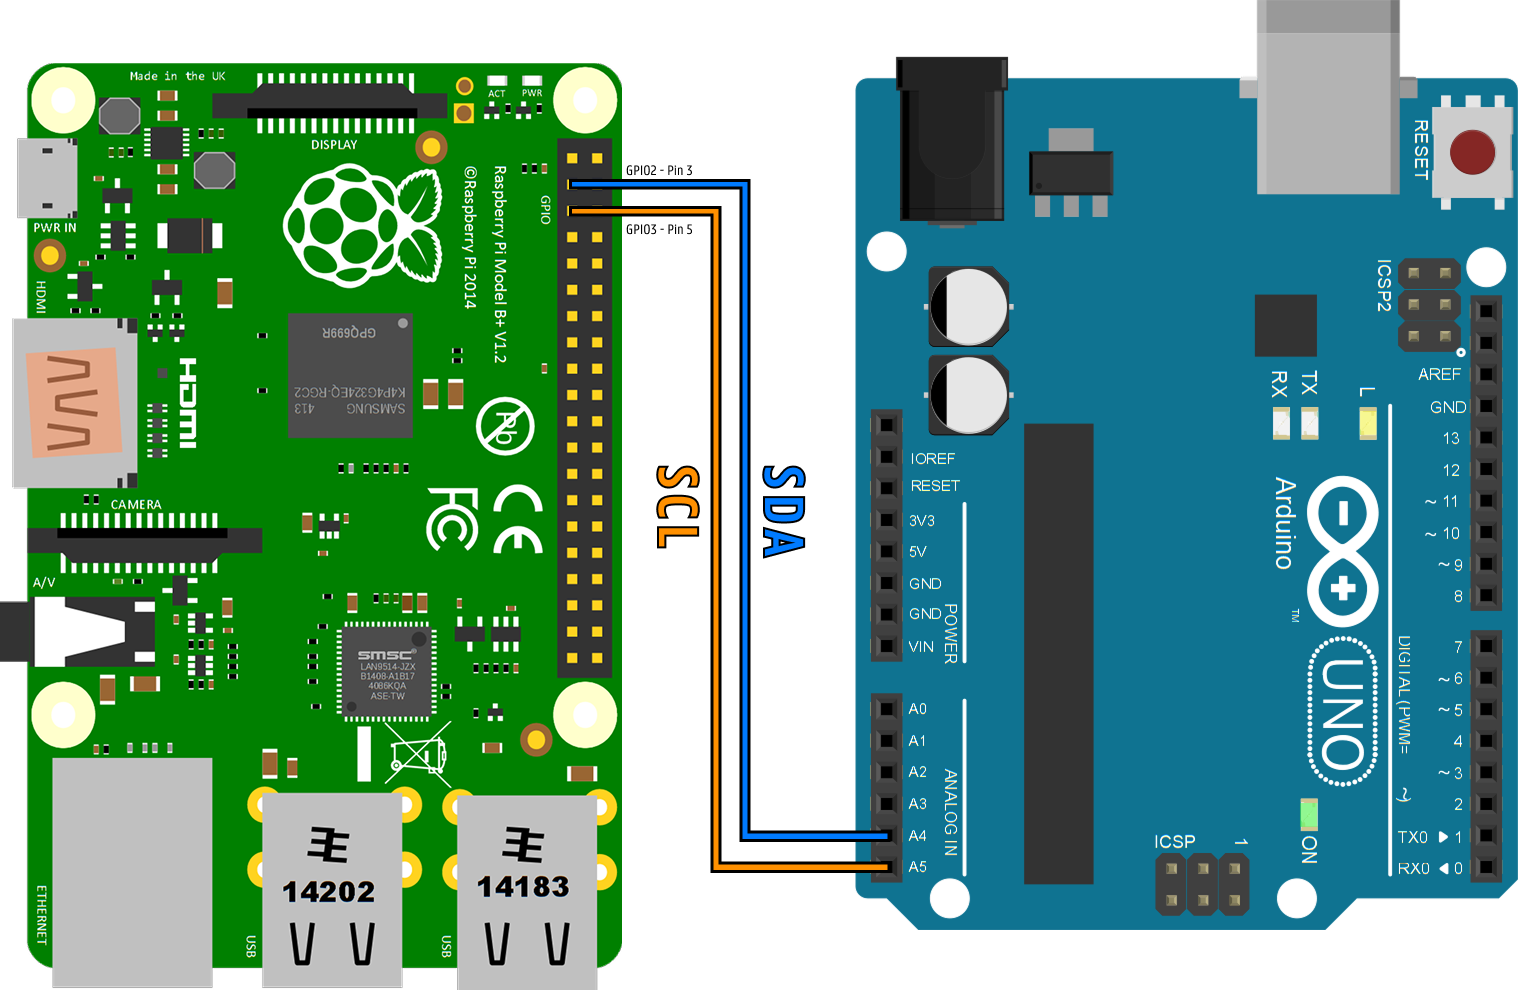
\includegraphics[width=0.7\textwidth]{images/HW_config.png}
	\caption{Hardware connection diagram. SDA: Pi pin 3 to Arduino A4; SCL: Pi pin 5 to Arduino A5. Ground cable connection was omitted for simplicity of the diagram, but uses Pi pin 6 to Arduino GND.}
	\label{fig:hw-connection}
\end{figure}

\subsection{Arduino Firmware Implementation}
\label{subsec:eval-setup-fw}

Two firmware versions were developed for different evaluation phases:

\subsubsection{Correctness Verification Firmware}
This firmware implements echo functionality for debugging. All I2C transactions are logged via USB serial, enabling transaction verification.

\subsubsection{Performance Testing Firmware}
For performance benchmarks, an optimized firmware version was deployed that eliminates serial communication overhead. Upon receiving any I2C write request, the Arduino responds with a fixed ``hello'' message (\texttt{0x68, 0x65, 0x6c, 0x6c, 0x6f}) for one subsequent read operation. This approach minimizes Arduino-side processing variability and keeps extra overhead to a minimum.

\subsection{Methodology}
\label{subsec:eval-setup-bench}

The evaluation follows a three-phase methodology to ensure correctness and robust measurement of latency and memory utilization.

\subsubsection{Phase 1: Correctness Verification}
Prior to profiling, functional correctness is verified by executing ping-pong operations across all implementations and confirming successful I2C transactions via Arduino serial monitor output.

\subsubsection{Phase 2: Performance Measurement}
Performance evaluation employs \textbf{Criterion.rs}, a statistical benchmarking framework that provides automatic outlier detection, distribution plotting, calculates achievable sample size prior to measurements during a warm-up phase and provides statistical insights post measurements\cite{criterion_rs}. The tool \texttt{cargo-criterion} provides machine-readable JSON output of those measurements, which allows us to also perform manual analysis and visualizations using Python/Jupyter.

The benchmark is divided into three different measurements, referred to as \textbf{Groups}. Each runtime gets evaluated over 100 samples according to the group's implementation:
\begin{itemize}
    \item \textbf{Runtime Setup:} Time to initialize runtime and prepare for I2C operations
    \item \textbf{Cold Execution:} A single ping-pong operation after a new runtime initialization
    \item \textbf{Hot Execution:} Repeated ping-pong operations in steady state
\end{itemize}

\subsubsection{Phase 3: Memory utilization}
A single binary is built to run memory utilization profiling across all the different runtimes, using DHAT~\cite{dhat_crate}. Two profilers are initialized, measuring Runtime Setup and Guest execution. A separate binary for each runtime is compiled to analyze the resulting binary sizes.

\section{Runtime Setup Performance Analysis}
\label{sec:eval-setup}

Runtime initialization represents a critical performance dimension, particularly for embedded devices deployed in scenarios where Time-to-First-Execution is crucial. This section analyzes the setup overhead for each runtime and discusses the implications for practical deployment scenarios.

While the native implementation is categorized under Runtime Setup, it does not involve any runtime initialization. Instead, it establishes a performance baseline by measuring the Linux I2C Stack overhead for opening the \texttt{/dev/i2c-1} device file. Since the \acrshort{wasm} implementations utilize the same underlying Linux I2C software stack, this baseline enables quantification of the additional overhead introduced purely by runtime instantiation when compared against the \acrshort{wasm} implementations.

Table~\ref{tab:wasm-setup} presents the initialization overhead for \acrshort{wamr} and Wasmtime implementations compared to the Native baseline. Figure~\ref{fig:wasm-setup-distribution} gives a visual representation.

\begin{table}[h]
    \centering
    \caption{Runtime Setup overhead comparison, showcasing absolute differences between implementations.}
    \label{tab:wasm-setup}
    \begin{tabular}{lccccc}
        \toprule
        \textbf{Implementation} & \textbf{Mean (µs)} & \textbf{Median (µs)} & \textbf{Std Dev (ns)} & \textbf{95\% CI (µs)} & \textbf{CI Range (µs)} \\
        \midrule
        Native      & 1.9466 & 1.9483 & 10.5846 & [1.9445 ; 1.9487] & 0.0042 \\
        WAMR        & 253.1126 & 253.1301 & 258.4145 & [253.0613 ; 253.1638] & 0.1025 \\
        Wasmtime    & 19,559.1592 & 19,559.8473 & 11,656.5225 & [19,556.8463 ; 19,561.4721] & 4.6258 \\
        \bottomrule
    \end{tabular}
\end{table}

\begin{figure}[h]
    \centering
    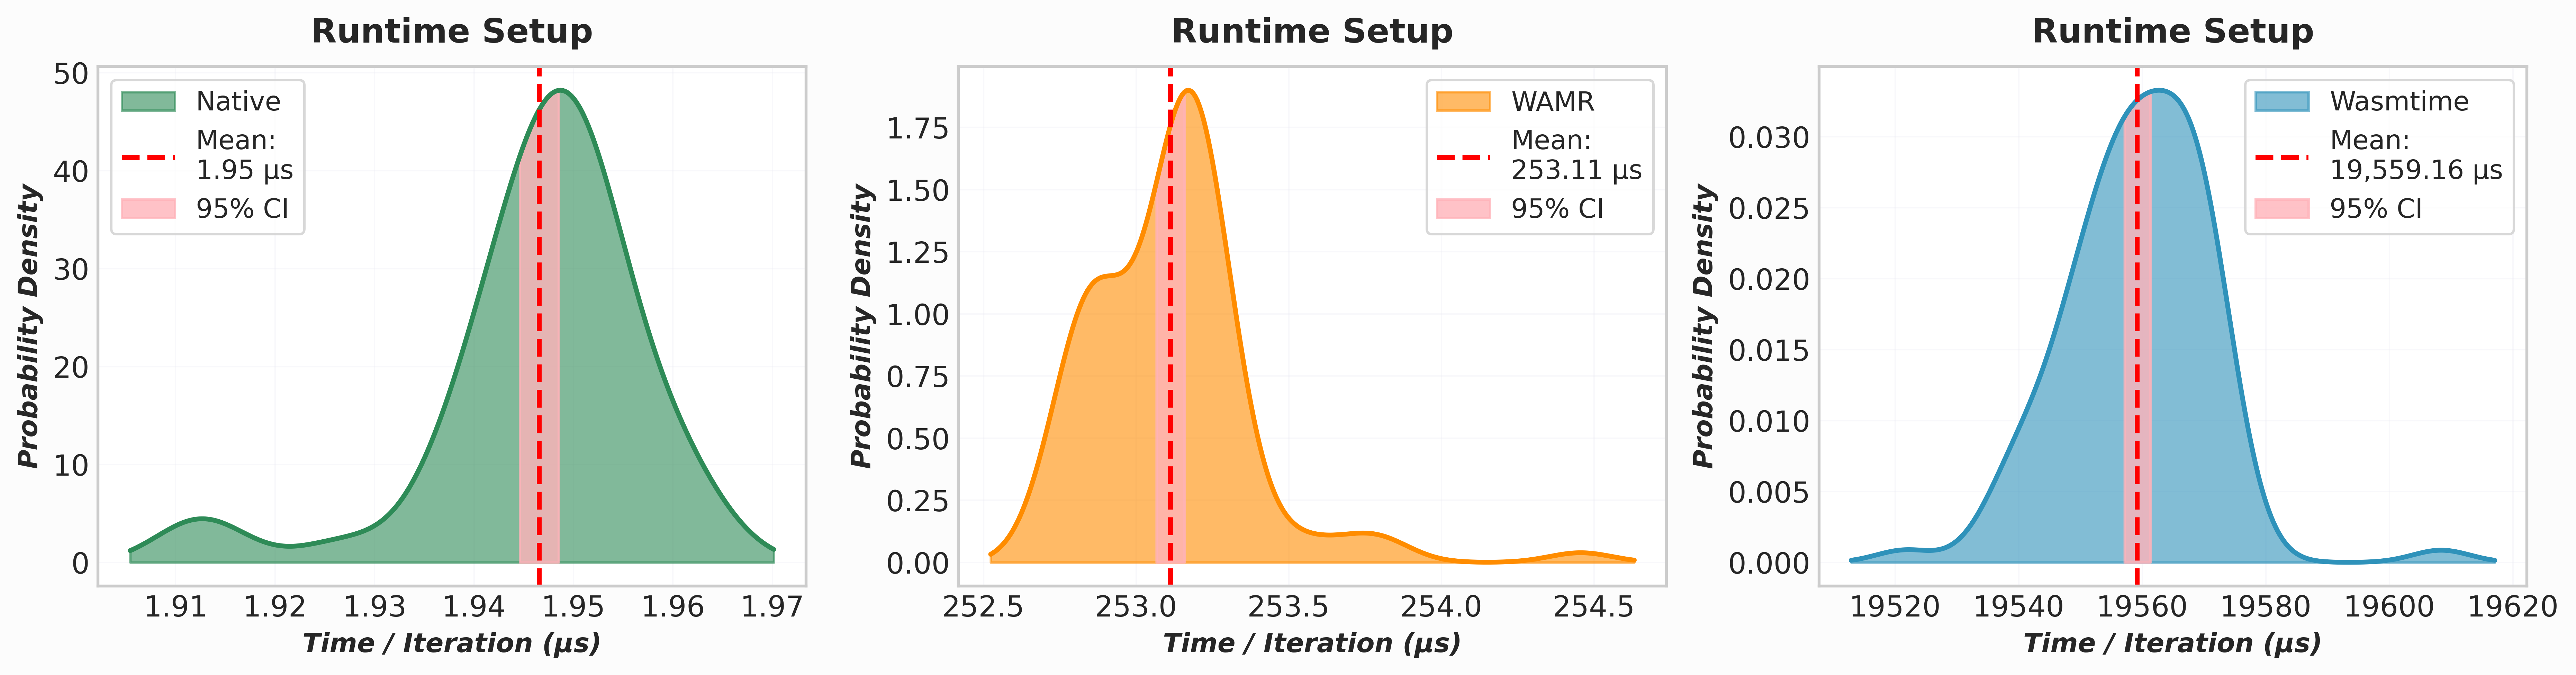
\includegraphics[width=0.9\textwidth]{images/setup-distribution}
    \caption{Distribution plots, showcasing relatively stable measurements.}
    \label{fig:wasm-setup-distribution}
\end{figure}

\subsection{Analysis}
The results reveal a dramatic performance disparity between the two WebAssembly runtimes. \acrshort{wamr} achieves setup initialization in approximately 253 μs, representing a 130x overhead compared to the native implementation. However, Wasmtime exhibits substantially higher initialization costs at 19.6 ms, creating a just over 10,000x overhead relative to the native implementation and a 77x overhead compared to the \acrshort{wamr} implementation. Figure~\ref{fig:wasm-setup-relative} gives a visualization of the dramatic differences.

\begin{figure}[h]
    \centering
    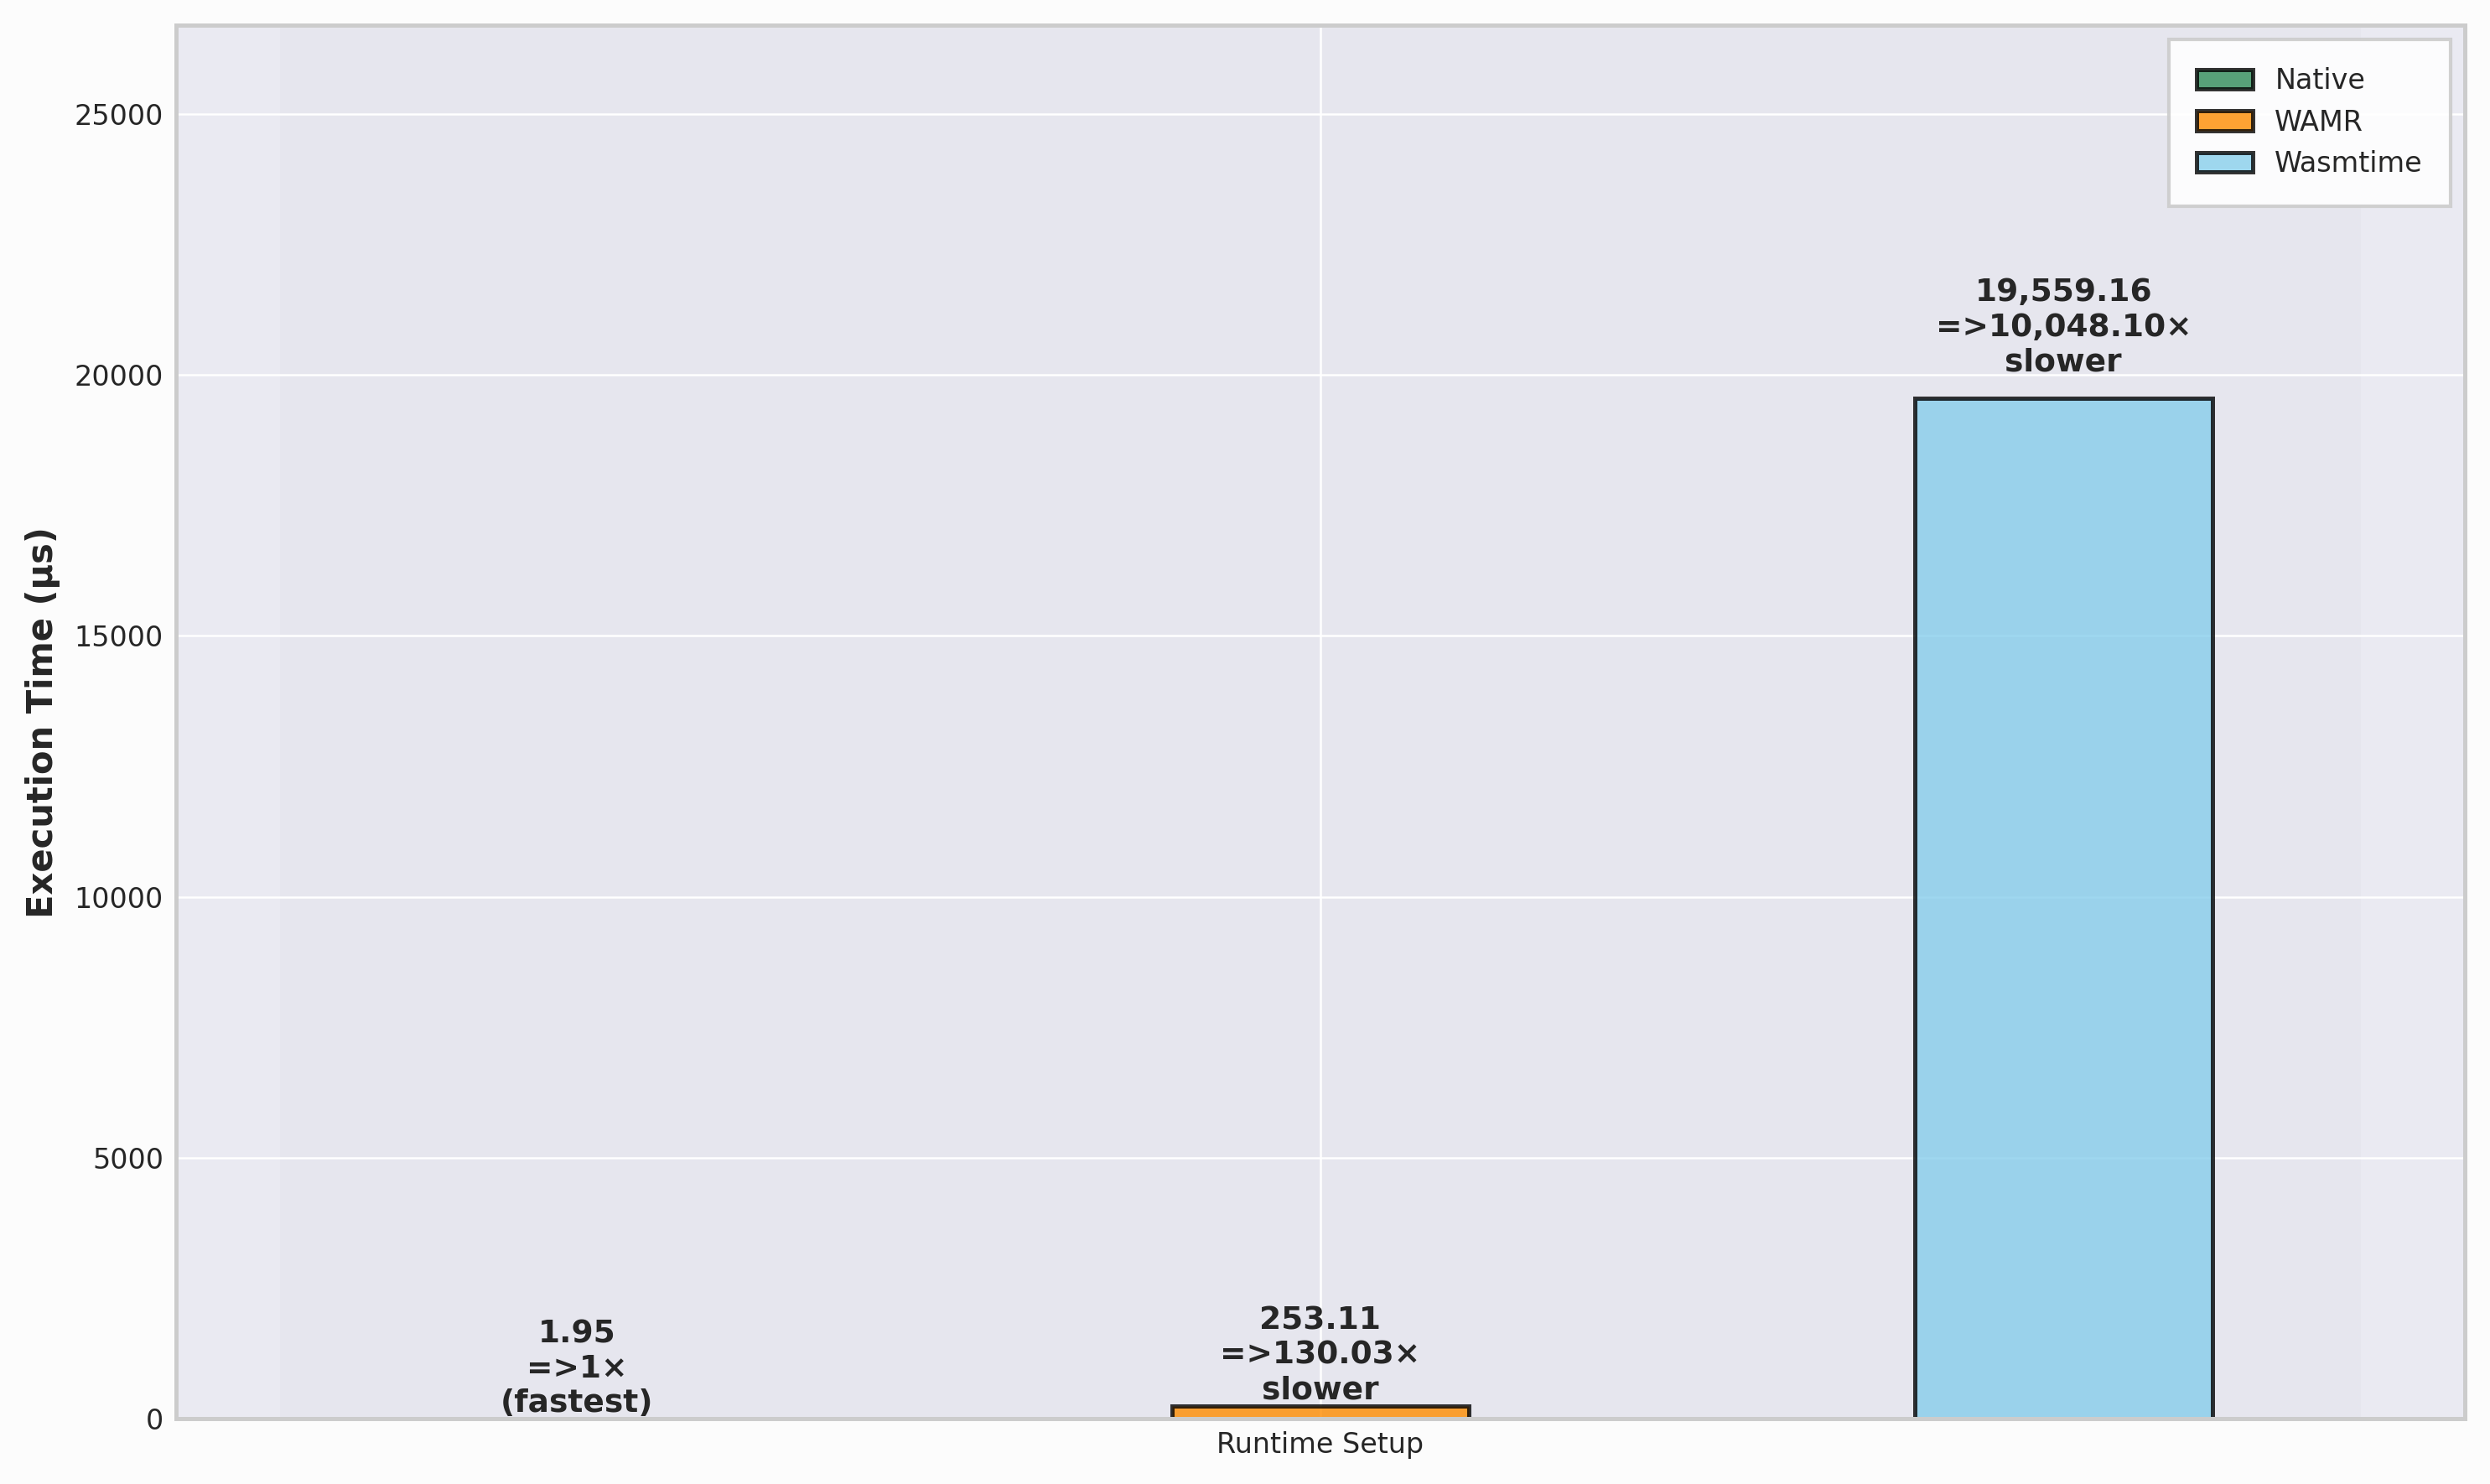
\includegraphics[width=0.9\textwidth]{images/setup_bars}
    \caption{Bar chart comparing Runtime Setup overhead, showcasing the much higher Wasmtime overhead for setting up the runtime.}
    \label{fig:wasm-setup-relative}
\end{figure}

\subsection{Embedded Application Implications}
\label{subsec:setup-implications}

These setup time characteristics have profound implications for embedded deployment patterns. For example:

\textbf{Ultra Low Power:} In some cases, Ultra Low Power devices leaving their duty cycle are completely turned off, making them lose their state. Setting up a new Wasmtime instance each time would take up too much power. In some extreme scenarios, even setting up \acrshort{wamr} could be too much overhead, but it would remain feasible in cases where the benefits of WebAssembly are favored.

\textbf{Real-time Systems:} Applications requiring deterministic startup behavior within millisecond constraints would exclude Wasmtime entirely, while \acrshort{wamr}'s sub-millisecond setup remains viable for many real-time scenarios.

\textbf{Long-running Applications:} Conversely, applications with infrequent instantiation (e.g., edge computing services) can amortize Wasmtime's setup cost over extended execution periods.

\section{Execution Performance Analysis}
\label{sec:eval-execution}

With runtime initialization complete, this section examines the steady-state execution performance for I2C operations, comparing cold (first-execution) and hot (repeated-execution) characteristics.

Table~\ref{tab:wasm-execution} compares execution performance between WAMR, Wasmtime, and Native for both Cold and Hot execution.

\begin{table}[h]
    \centering
    \caption{WebAssembly Execution Performance Comparison}
    \label{tab:wasm-execution}
    \begin{tabular}{llcccc}
        \toprule
        \textbf{Execution} & \textbf{Implementation} & \textbf{Mean (µs)} & \textbf{Median (µs)} & \textbf{Std Dev (ns)} & \textbf{95\% CI (µs)} \\
        \midrule
                & Native    & 594.5275 & 594.5636 & 281.8579 & [594.4715 ; 594.5834] \\
        Cold    & WAMR      & 1,211.0415 & 1,210.9849 & 5,144.4222 & [1,210.0207 ; 1,212.0622] \\
                & Wasmtime  & 1,301.8975 & 1,300.5868 & 4,895.5251 & [1,300.9262 ; 1,302.8689] \\
        \hline
                & Native    & 589.0368 & 589.0307 & 69.9196 & [589.0230 ; 589.0507] \\
        Hot     & WAMR      & 1,185.4778 & 1,185.8310 & 673.0608 & [1,185.3442 ; 1,185.6113] \\
                & Wasmtime  & 1,184.4430 & 1,184.2941 & 522.5048 & [1,184.3393 ; 1,184.5467] \\
        \bottomrule
    \end{tabular}
\end{table}

\begin{figure}[h]
    \centering
    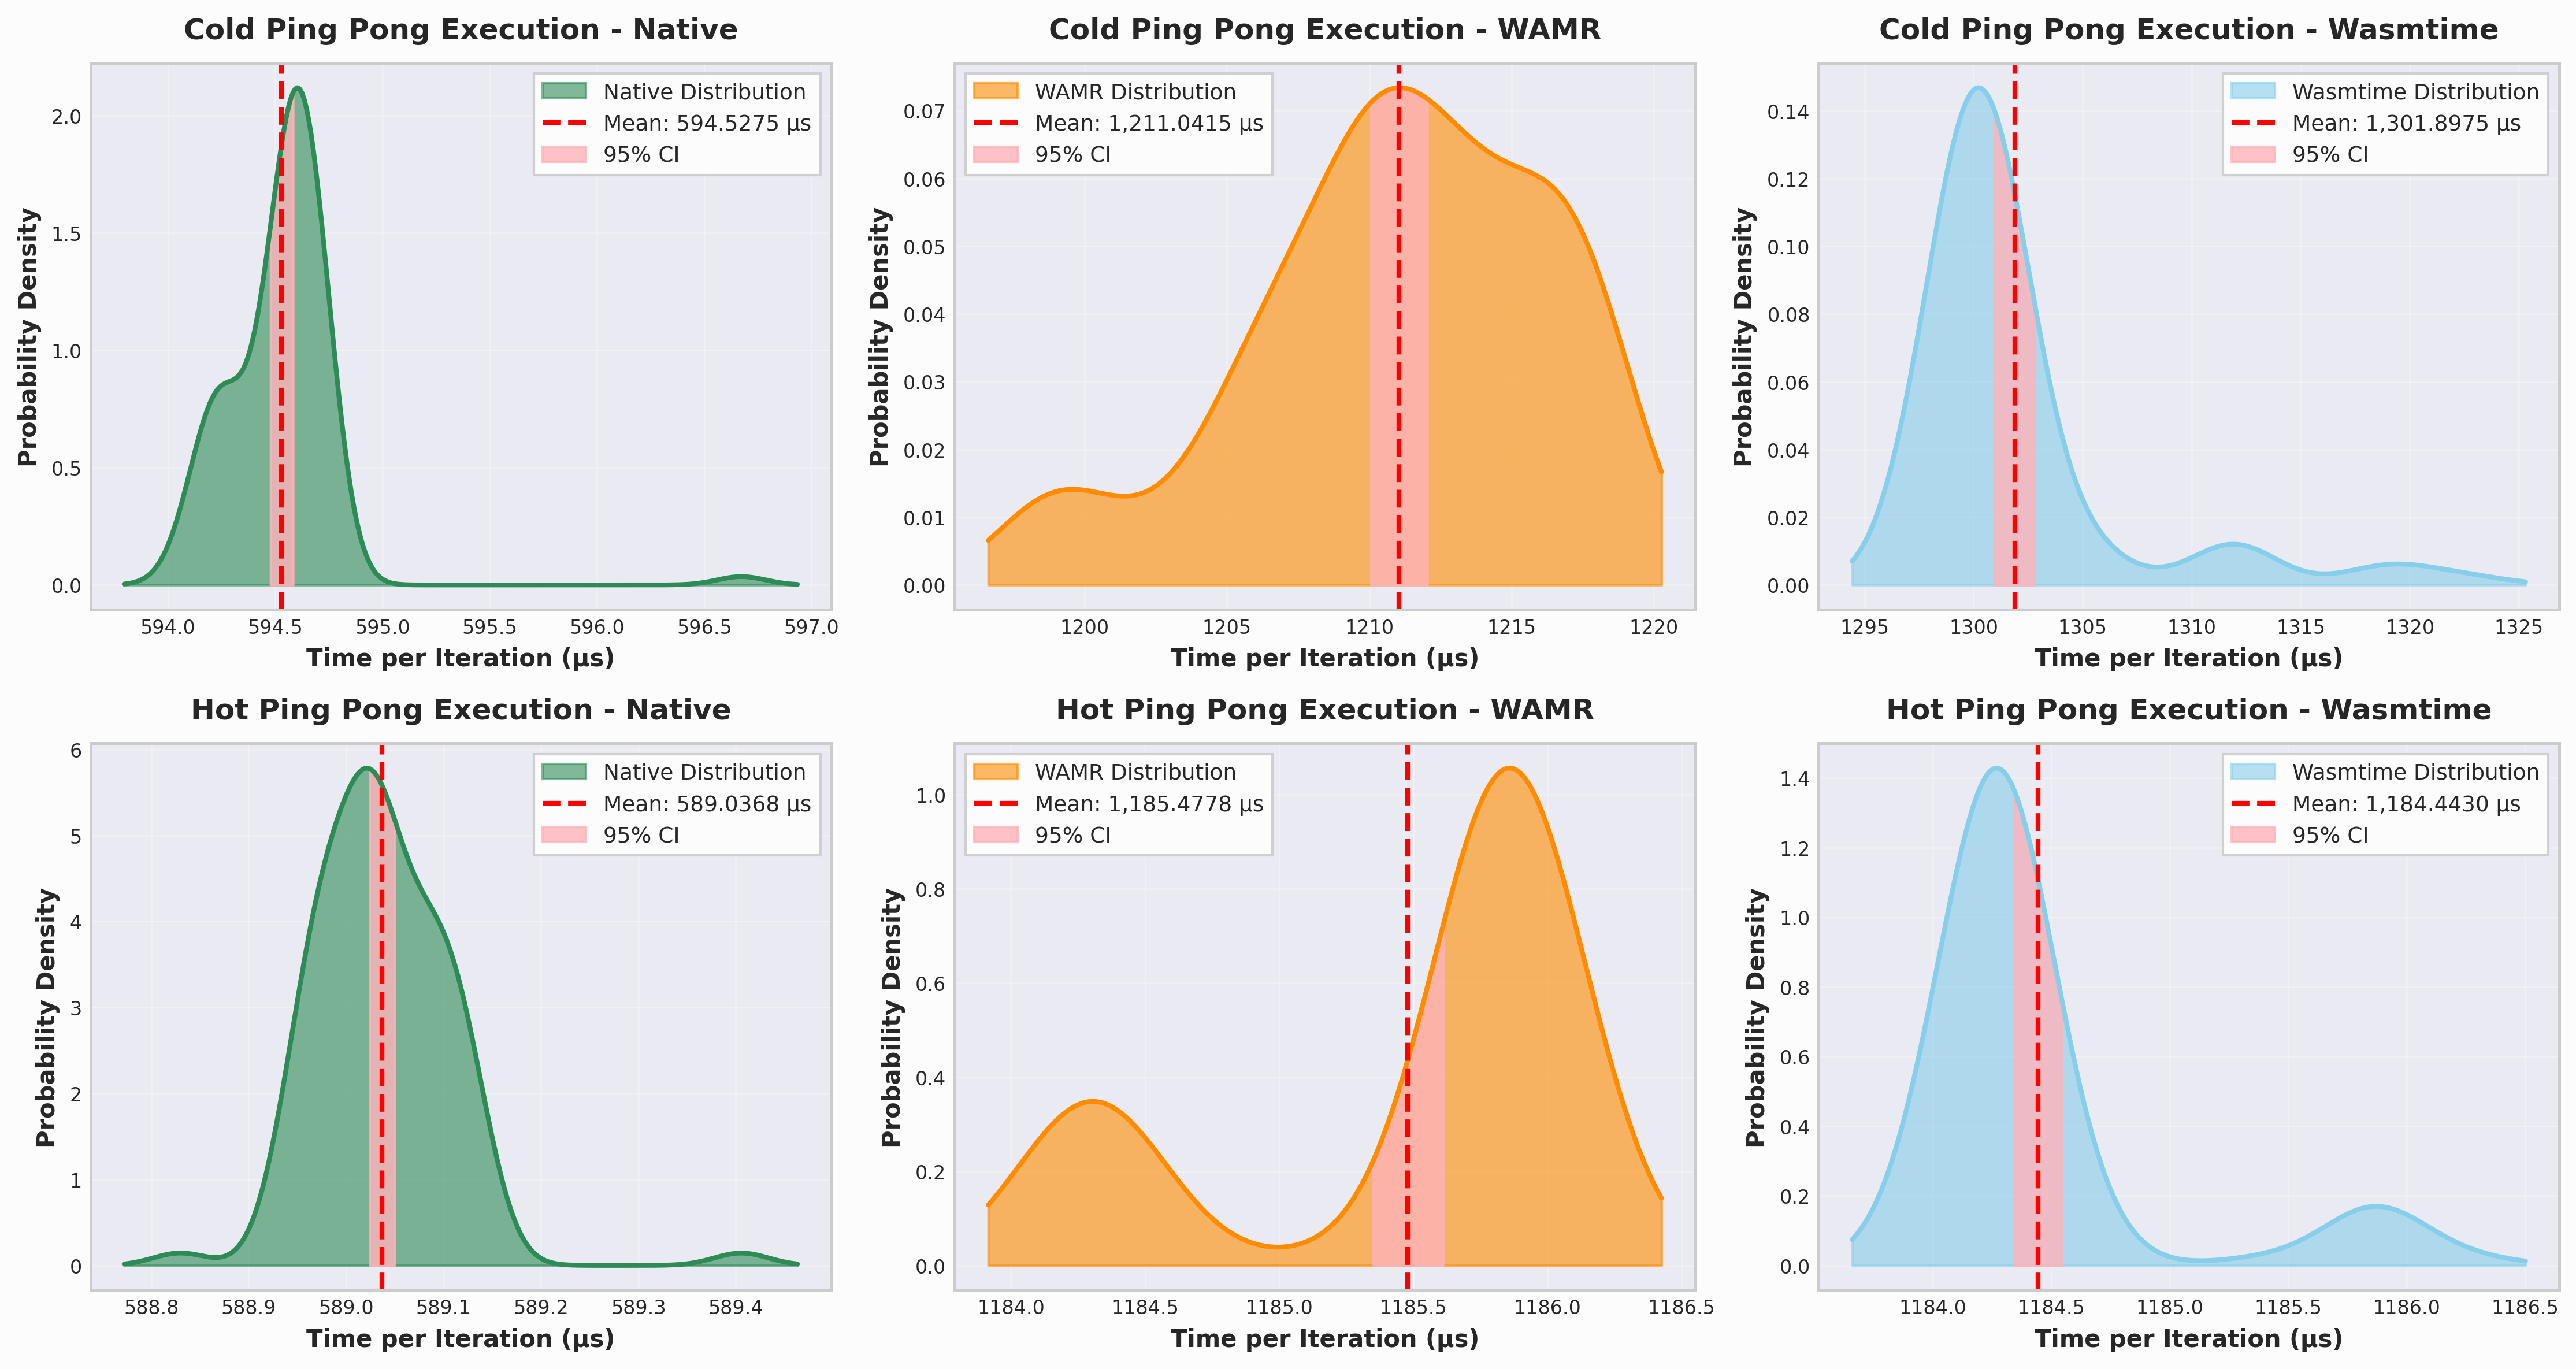
\includegraphics[width=0.9\textwidth]{images/execution-distribution}
    \caption{Distribution plots, showcasing stability of the measurements.}
    \label{fig:wasm-setup-distribution}
\end{figure}

\subsection{Analysis}

\begin{figure}[h]
    \centering
    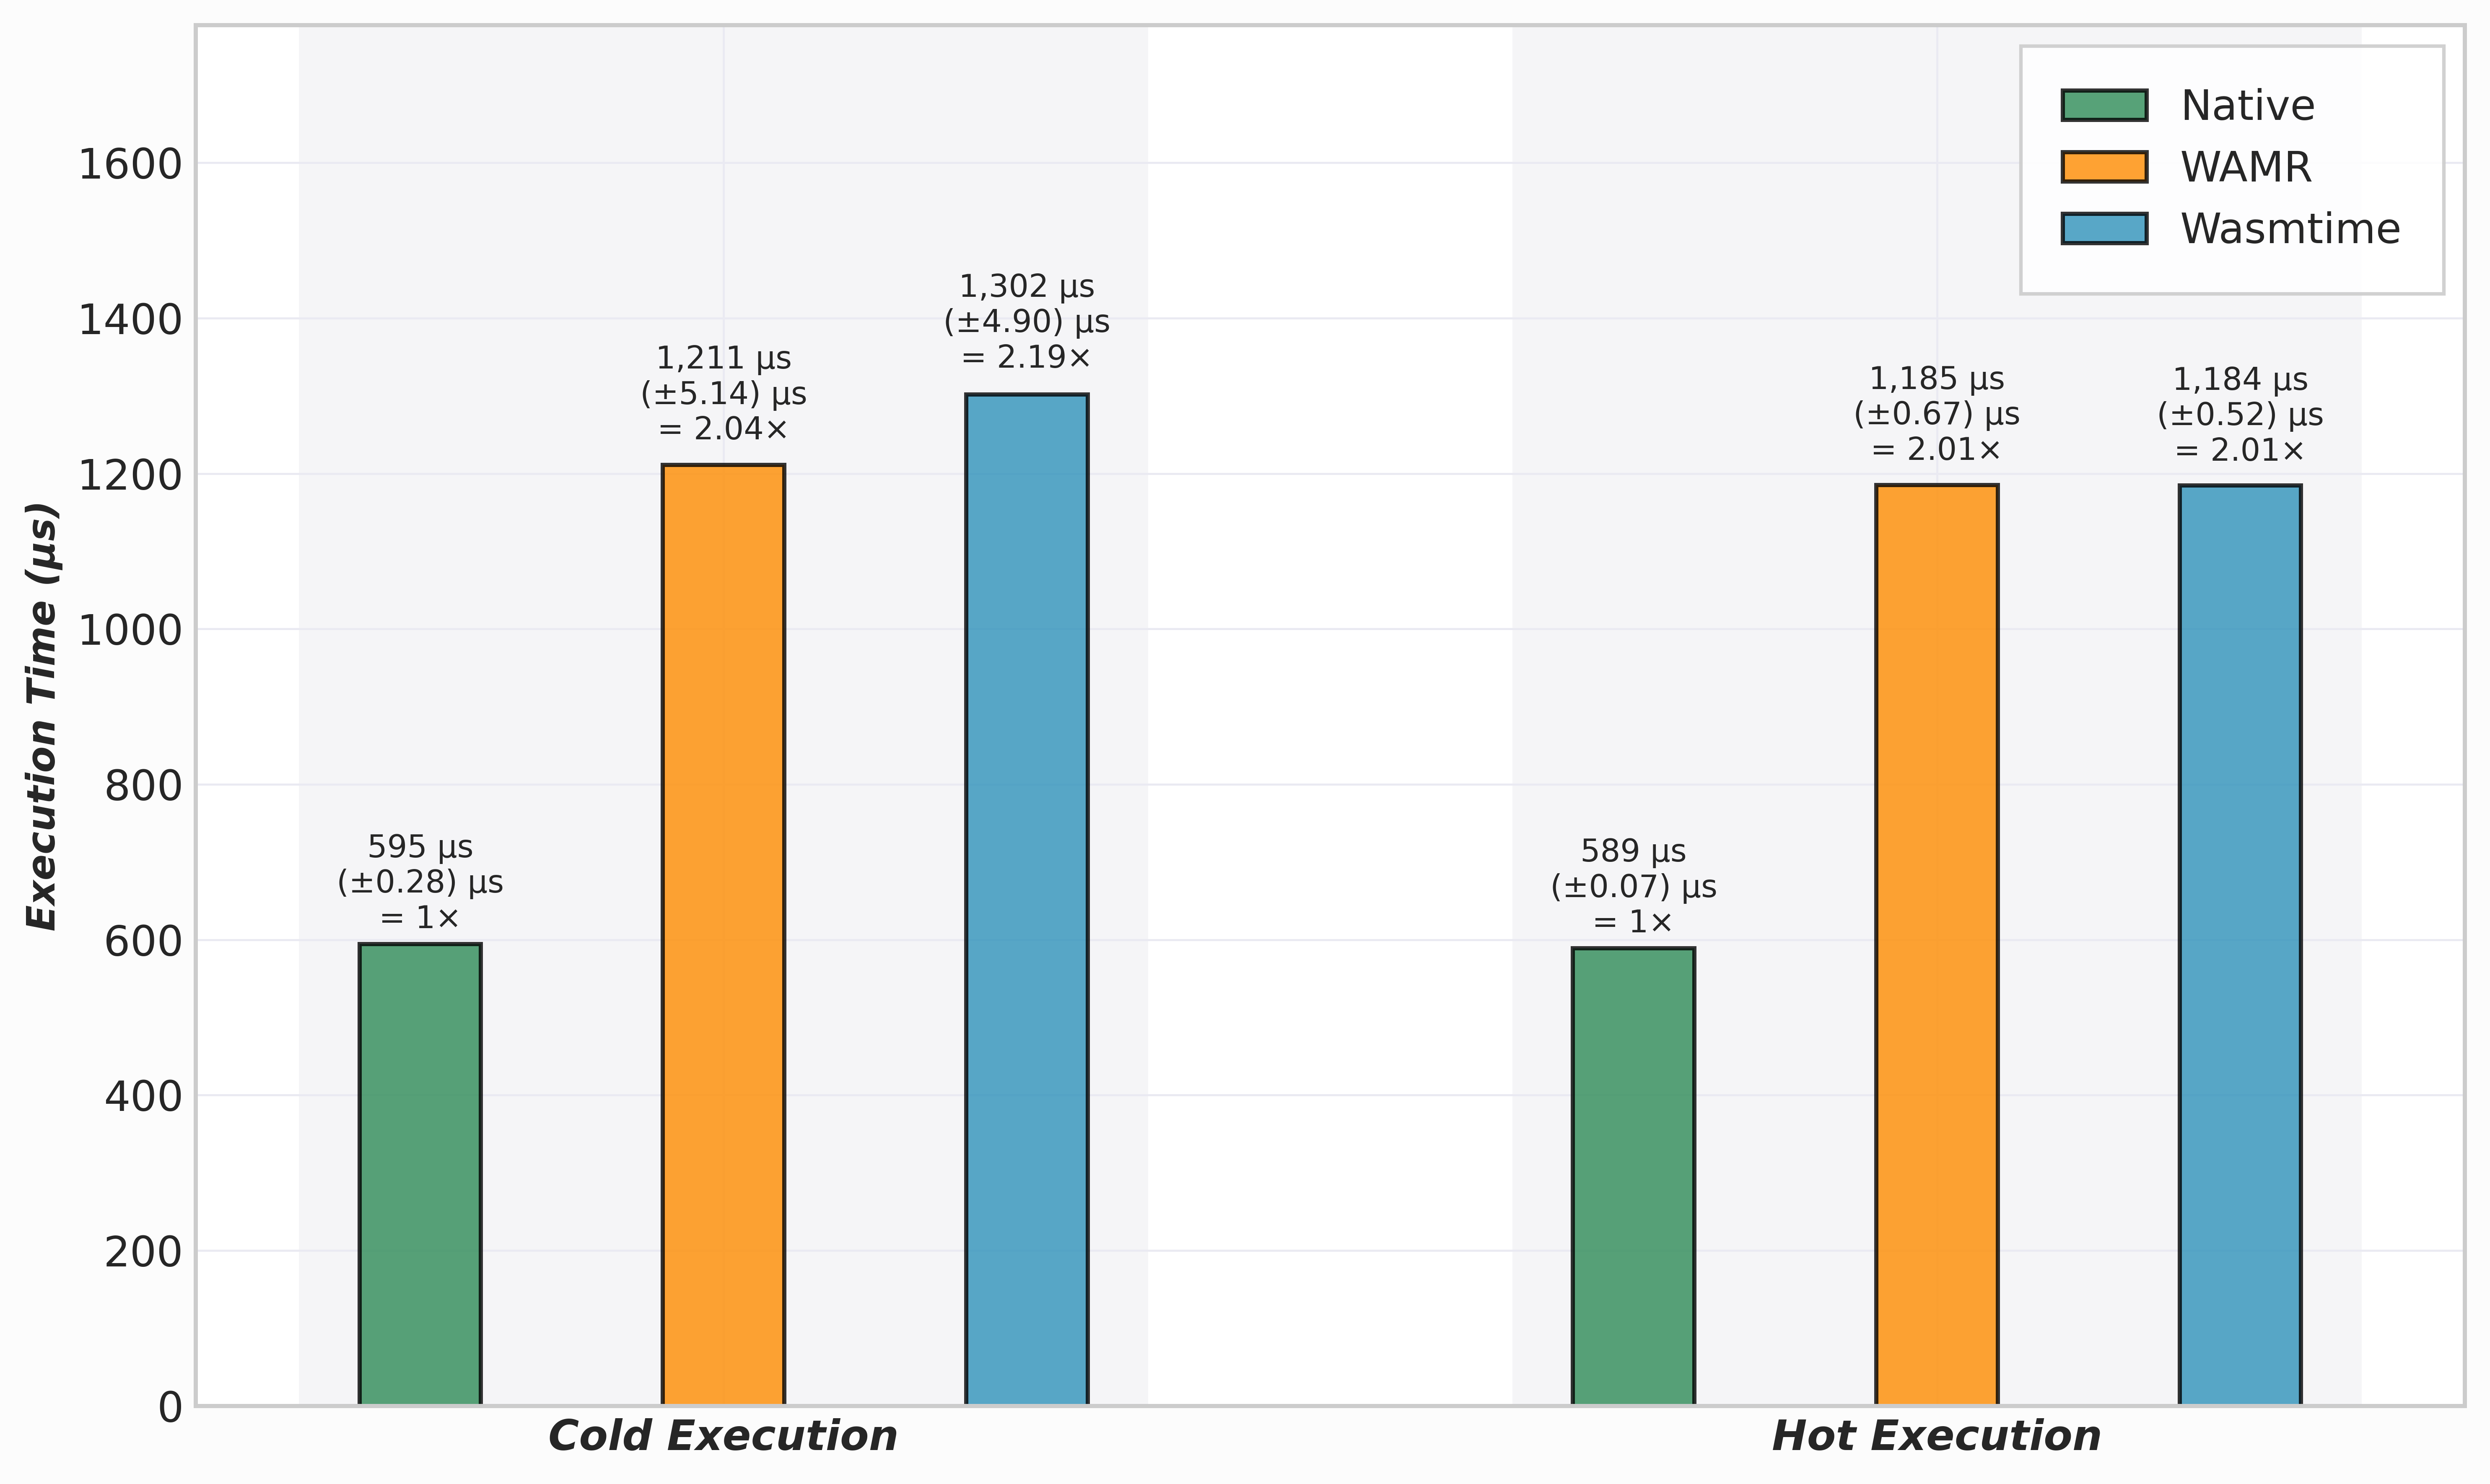
\includegraphics[width=1.0\textwidth]{images/wasm-execution-rel}
    \caption{Execution Performance Comparison: Native vs \acrshort{wamr} vs Wasmtime}
    \label{fig:wasm-execution-relative}
\end{figure}

\begin{enumerate}
    \item \textbf{Convergent Steady-State Performance:} Both WAMR and Wasmtime achieve remarkably similar hot execution performance with a 2x native overhead, despite their architectural differences.
    
    \item \textbf{Cold/Hot Differences:} Minimal cold/hot differences for WAMR (2.1\% improvement), with Wasmtime showing moderate optimization benefits (9.0\% improvement), suggesting some caching or similar optimization effects.
    
    \item \textbf{Consistent WebAssembly Overhead:} Both implementations exhibit approximately 2x overhead compared to native execution, representing the cost of WebAssembly instruction execution and host function call marshalling.
\end{enumerate}

\subsection{Performance Variability Assessment}
\label{subsec:eval-execution-variability}

Table~\ref{tab:variability} presents Coefficient of Variation (CV) metrics to assess performance consistency across implementations. Figure~\ref{fig:variability-comparison}

\begin{table}[h]
    \centering
    \caption{Performance Variability Comparison (Coefficient of Variation)}
    \label{tab:variability}
    \begin{tabular}{lccc}
    \toprule
    \textbf{Implementation} & \textbf{Setup CV (\%)} & \textbf{Cold Exec CV (\%)} & \textbf{Hot Exec CV (\%)} \\
    \midrule
    Native       & 0.5438 & 0.0474 & 0.0119 \\
    WAMR         & 0.1021 & 0.4248 & 0.0568 \\
    Wasmtime     & 0.0596 & 0.3760 & 0.0441 \\
    \bottomrule
    \end{tabular}
\end{table}

\begin{figure}[h]
    \centering
    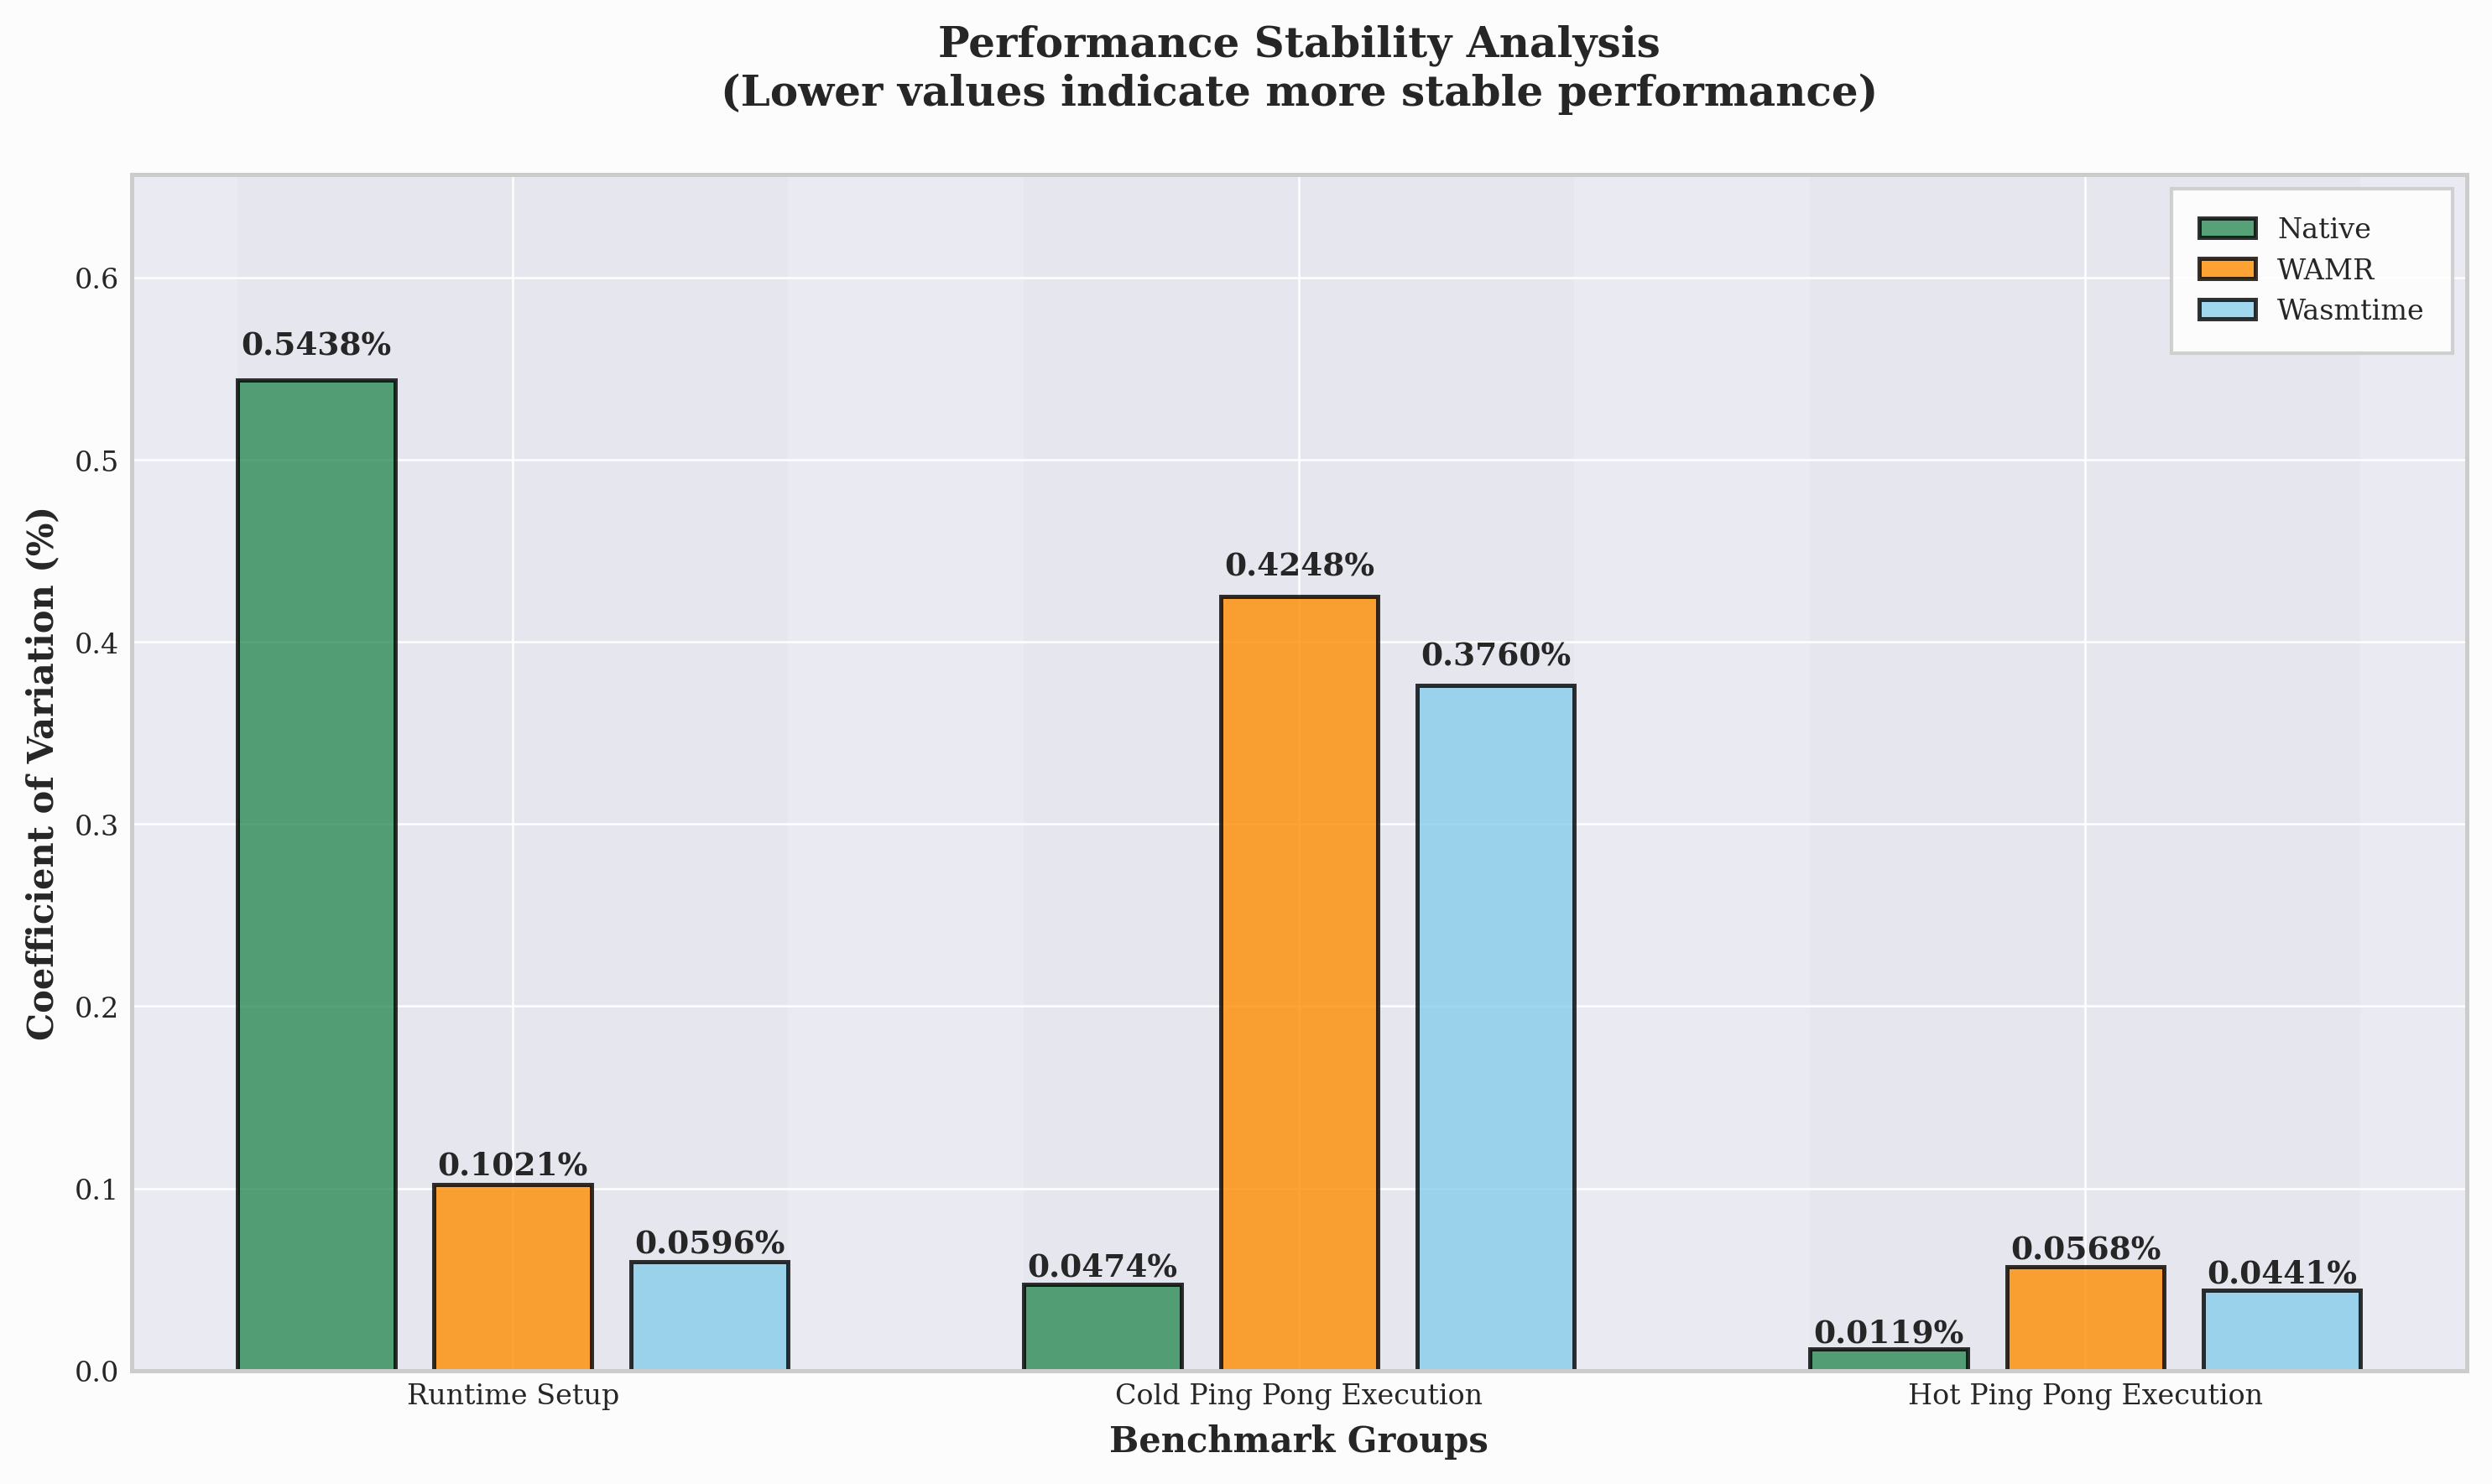
\includegraphics[width=0.9\textwidth]{images/variability-comparison}
    \caption{Comparison of calculated Coefficient of Variation across all implementations}
    \label{fig:variability-comparison}
\end{figure}

The performance variability analysis reveals distinct consistency patterns across the three implementations. During the setup phase, the native implementation exhibits the highest variability (0.54\% CV), suggesting that direct hardware initialization is less predictable or stable, while Wasmtime demonstrates the most consistent setup behavior (0.06\% CV). This pattern reverses during cold execution, where both WebAssembly runtimes show significantly higher variability (WAMR: 0.42\%, Wasmtime: 0.38\%) compared to the native implementation (0.047\%). This increased variability can be attributed to the complex initialization and optimization processes within the WebAssembly runtimes during first execution. However, during hot execution, all implementations converge to low variability levels, with the native implementation achieving the highest consistency (0.012\% CV), followed by Wasmtime (0.044\%) and WAMR (0.057\%). Importantly, all Coefficient of Variation values remain well below 1\%, indicating that despite relative differences between implementations, all approaches demonstrate excellent measurement consistency and predictable performance characteristics.

\section{Memory Usage Analysis}
\label{sec:eval-memory}

Memory consumption patterns provide critical insights for embedded applications with constrained resources. This section analyzes heap allocation behavior during both runtime setup and execution phases using DHAT profiling.

\subsection{Runtime Setup}
\label{subsec:memory-setup}

Table~\ref{tab:memory-setup} presents memory allocation characteristics during runtime initialization, revealing the resource requirements for each implementation approach.

\begin{table}[h]
    \centering
    \caption{Memory Usage During Runtime Setup}
    \label{tab:memory-setup}
    \begin{tabular}{lccc}
        \toprule
        \textbf{Implementation} & \textbf{Total (bytes)} & \textbf{Peak (bytes)} & \textbf{Blocks (count)} \\
        \midrule
        Native        & 10          & 10        & 1 \\
        WAMR          & 10,124      & 10,080    & 16 \\
        Wasmtime      & 14,247,171  & 2,716,728 & 16,686 \\
        \bottomrule
    \end{tabular}
\end{table}

\subsubsection{Analysis}

The memory allocation patterns during runtime initialization reveal fundamental architectural differences between the implementations. The native implementation establishes a minimal baseline with just 10 bytes allocated, reflecting direct hardware access without abstraction overhead.

WAMR demonstrates embedded-friendly resource consumption, requiring approximately 10KB across 16 allocation blocks. This three-order-of-magnitude increase over native remains acceptable for most embedded systems, particularly given that 99.6\% of allocated memory persists throughout the runtime lifecycle—indicating efficient, stable memory management without excessive allocation churn.

Wasmtime's memory profile reflects its sophisticated execution engine architecture. While total allocations reach 14.2MB during initialization, the runtime maintains only 2.7MB at peak usage. This 81\% temporary allocation ratio reveals intensive memory operations during JIT compilation and module optimization. The 16,686 allocation blocks (over 1,000x more than WAMR) further illustrate the complexity of component model instantiation and type system initialization. Most importantly, Wasmtime's peak memory usage crosses the RAM limitations of both the ESP32-C3 (400KB) and the Nucleo (256KB) of the Portability Criteria from Table~\ref{tab:portability_criteria_specs}. Further optimization strategies were not researched, so will not be discussed.

These patterns directly impact deployment feasibility: WAMR's 10KB footprint fits comfortably within typical embedded constraints (even sub-MB microcontrollers), while Wasmtime's multi-megabyte requirements restrict it to more capable embedded Linux platforms. The correlation between memory complexity and setup time (77x difference) suggests that memory allocation overhead contributes significantly to initialization latency.

\section{Binary Size}



% TODO: decide on OLD or new content
% \subsubsection{Setup Memory Analysis:}
% The memory consumption analysis during runtime setup reveals dramatic differences in resource requirements across implementations, with implications spanning several orders of magnitude. The \textbf{native }implementation demonstrates minimal memory overhead, allocating only 10 bytes in a single allocation block, reflecting the direct hardware access approach with virtually no abstraction layer overhead. This establishes an extremely lean baseline that showcases the efficiency of direct I2C library usage.

% \textbf{WAMR} presents a moderate memory footprint, consuming 10,124 bytes (approximately 10KB) total allocation with a peak usage of 10,080 bytes across 16 allocation blocks. This represents a three-order-of-magnitude increase compared to the native implementation, yet remains within reasonable bounds for embedded applications. The close alignment between total and peak memory usage (10,124 vs 10,080 bytes) demonstrates that WAMR maintains most allocated memory throughout the setup process, indicating a relatively stable memory profile with minimal temporary allocations.

% In stark contrast, \textbf{Wasmtime} exhibits substantially higher memory requirements, allocating 14,247,171 bytes (approximately 14.2 MB) total across 16,686 allocation blocks during setup. However, the peak memory usage of 2,716,728 bytes (approximately 2.7 MB) reveals that roughly 81\% (\(\frac{Total-Peak}{Total}\)) of allocated memory consists of temporary allocations that are freed during the setup process. This pattern indicates intensive memory churning during runtime initialization, likely associated with JIT compilation, module loading, and optimization processes inherent to Wasmtime's sophisticated execution engine.

% The allocation \textbf{block count provides additional insight} into memory management patterns. While the native implementation requires only a single allocation, WAMR uses 16 blocks, suggesting modular memory organization. Wasmtime's 16,686 allocation blocks demonstrate the complex memory management required for its advanced runtime features, including component model support and aggressive optimization strategies.

% From an \textbf{embedded systems perspective}, these results highlight critical deployment considerations. WAMR's 10 KB memory overhead remains feasible for many embedded applications, while Wasmtime's multi-megabyte requirements may exceed available memory in resource-constrained environments. The memory consumption patterns also correlate with the observed setup performance differences, where Wasmtime's extensive memory allocation activity contributes to its longer initialization times, while WAMR's moderate memory footprint aligns with its faster setup performance.

\subsection{Execution}

Table~\ref{tab:memory-execution} presents memory allocation characteristics during the execution of the Ping-Pong routine, revealing the resource requirements for each implementation approach.

\begin{table}[H]
    \centering
    \caption{Memory Usage During Ping-Pong Execution}
    \label{tab:memory-execution}
    \begin{tabular}{lrrr}
        \toprule
        \textbf{Implementation} & \textbf{Total (bytes)} & \textbf{Peak (bytes)} & \textbf{Blocks (count)} \\
        \midrule
        Native        & 16   & 16  & 1 \\
        WAMR          & 327  & 311 & 6 \\
        Wasmtime      & 416  & 347 & 10 \\
        \bottomrule
    \end{tabular}
\end{table}

\subsubsection{Analysis}

Both runtimes demonstrate remarkable efficiency: WAMR requires 327 bytes across 6 allocations, while Wasmtime uses 416 bytes across 10 allocations --- a negligible 89-byte difference despite their architectural disparities. Compared to the 16-byte native baseline, this represents approximately 20-26x overhead, primarily attributable to WASI interface marshalling and guest-host communication buffers.

The minimal peak-to-total allocation differences (WAMR: 5\%, Wasmtime: 17\%) indicate stable execution without memory leaks or excessive temporary allocations. This efficiency validates both runtimes for long-running embedded applications where thousands of I2C operations must execute within constrained memory budgets.

Critically, these results demonstrate that the substantial initialization costs --- particularly Wasmtime's 14.2MB --- do not translate to proportional execution overhead. Once initialized, both runtimes operate within hundreds of bytes, making the initialization cost a one-time investment that can be amortized across the application lifetime.

% TODO: Decide on OLD or new content
% \subsection{Execution Memory Profiling}
% \label{subsec:memory-execution}

% Table~\ref{tab:memory-execution} analyzes memory allocation patterns during ping-pong execution, focusing on runtime overhead and potential memory leaks.



% \subsubsection{Execution Memory Efficiency:}
% The memory consumption during ping-pong execution reveals the incremental memory overhead required for actual I2C operation execution, measured independently from the established runtime footprint. Since these measurements capture only the additional allocations occurring during guest function execution (after runtime initialization is complete), they provide insight into the operational memory efficiency of each approach.

% The \textbf{native} implementation requires 16 bytes in a single allocation block specifically for executing the ping-pong I2C operation. This represents the pure memory cost of the I2C transaction, including data buffers and operation state management without any runtime abstraction overhead.

% \textbf{WAMR} demonstrates remarkably efficient execution memory usage, requiring only 327 bytes total with a peak usage of 311 bytes across 6 allocation blocks. This modest overhead represents the additional memory needed by the WebAssembly runtime to execute the guest function, manage the WASI I2C interface calls, and handle parameter marshaling between the WebAssembly module and the host I2C implementation. The minimal difference between total and peak allocations (16 bytes, approximately 4.9\%) indicates that WAMR maintains very stable memory usage during execution with virtually no temporary allocation churn.

% \textbf{Wasmtime} requires 416 bytes total allocation with a peak usage of 347 bytes distributed across 10 allocation blocks for execution. While this represents the highest overhead among the implementations, the absolute increment remains modest at approximately 26 times the native requirement and only 1.27 times the WAMR requirement. The 69 bytes difference between total and peak usage (16.6\%) suggests slightly more dynamic memory management during execution, potentially related to component model overhead.

% These results are particularly significant because they demonstrate that \textbf{both WebAssembly runtimes achieve very efficient steady-state execution}. After absorbing the substantial initialization costs (especially Wasmtime's 14.2MB setup overhead), the incremental memory required for actual I2C operations remains in the hundreds of bytes range. This profile makes both runtimes highly suitable for embedded applications performing repeated I2C operations, where the setup cost can be amortized and the per-operation overhead remains minimal.
\chapter*{Conclusion}
\chaptermark{Conclusion}
\addcontentsline{toc}{chapter}{Conclusion}
\label{chap:conclusion}

This thesis addressed the critical challenge of bridging WASI Preview 2 I2C interface specifications with resource-constrained embedded systems through a comprehensive Preview 1 implementation ecosystem. By developing manual bindings, runtime integrations, and comparative frameworks, this work advances the WASI I2C standardization effort while providing empirical insights into WebAssembly runtime performance trade-offs in embedded environments.

% \section*{Research Contributions and Summary}
% \label{sec:research-summary}

% This investigation makes several key contributions to embedded WebAssembly deployment and WASI I2C standardization. The manual Rust bindings library demonstrates successful translation of WIT-defined interface semantics to Preview 1's function call mechanisms while preserving type safety and error handling. The complete implementation ecosystem establishes practical deployment strategies for resource-constrained embedded systems.

% The empirical evaluation provides the first rigorous performance comparison between WAMR and Wasmtime for embedded I2C applications, establishing quantitative baselines for startup latency, memory utilization, and resource efficiency. Most importantly, this work directly supports the WASI I2C proposal's progression toward Phase 3 standardization by demonstrating embedded system compatibility --- a previously unaddressed requirement.

\section*{Research Questions Answered}
\label{sec:research-questions-answered}

\textbf{Research Question 1: How can the WASI Preview 2 I2C interface be effectively adapted for WASI Preview 1 environments while maintaining functional compatibility with the standardized Preview 2 specification?}

This thesis demonstrates successful adaptation of Preview 2 interface semantics to Preview 1 environments through manual binding implementation. The \texttt{wasip1-i2c-lib} library successfully translates resource-based I2C controller management, error handling, and simple communication patterns to Preview 1's function call mechanisms while maintaining type safety and functional equivalence with Preview 2 implementations. This validates that the interface can target both modern component model environments and resource-constrained systems.

\textbf{Research Question 2: How do Preview 1 and Preview 2 approaches compare in terms of developer experience, maintainability, and implementation complexity?}

The analysis reveals fundamental trade-offs between developer convenience and deployment flexibility. Preview 2's automatic code generation provides superior developer experience through \texttt{wit-bindgen}, while Preview 1 approaches offer advantages in embedded contexts: implementation transparency, runtime simplicity, deployment flexibility with lightweight runtimes like WAMR, and optimization opportunities. The development effort for manual Preview 1 bindings represents a significant investment compared to automatic generation, but enables deployment in resource-constrained environments where Preview 2 approaches are infeasible.

\textbf{Research Question 3: What are the performance implications of WASI Preview 2 compared to Preview 1 for embedded I2C applications?}

The empirical evaluation reveals dramatic performance differences with clear embedded deployment implications. WAMR demonstrates 77x faster startup (253μs vs 19,559μs) and dramatically lower memory requirements (10KB vs 2.7MB peak usage). Wasmtime's memory usage exceeds RAM limitations of ESP32-C3 and Nucleo F412ZG platforms, limiting deployment to capable platforms. Both runtimes achieve efficient steady-state execution with both a 2x latency overhead compared to native and acceptable memory consumption (WAMR: 327 bytes, Wasmtime: 416 bytes). These findings establish WAMR as viable for resource-constrained applications while Wasmtime remains viable for more capable (embedded) platforms. WAMR is therefore able to meet the requirements defined by the Portability Criteria.

\section*{Impact on WASI I2C Standardization}
\label{sec:standardization-impact}

This work provides advances of the WASI I2C proposal --- toward Phase 3 requirements --- by addressing critical embedded system compatibility.

The advancements of the proposal to its current state revealed dependency on WASI Preview 2 and component model architecture that created embedded deployment barriers. \textbf{The developed Preview 1 compatibility} from this research eliminates these barriers by demonstrating that the WASI I2C interface \textbf{accommodates resource-constrained environments without compromising functionality}. The successful WAMR integration proves lightweight WebAssembly runtimes can provide I2C hardware access while maintaining interface semantic integrity.

\textbf{Key standardization contributions} include embedded compatibility demonstration, performance baselines for deployment decisions, and a complete Preview 1 reference implementation. Beyond I2C-specific contributions, this work establishes approaches for adapting WASI Preview 2 interfaces defined in WIT-files to embedded environments, providing methodology templates for other hardware interfaces (e.g., SPI, PWM, UART).

\section*{Limitations and Threats to Validity}
\label{sec:limitations}

This investigation acknowledges several limitations that constrain the generalizability and scope of findings:

\textbf{Workload Scope:} The evaluation focuses exclusively on the simple ping-pong I2C operations, which may not represent the complexity of production embedded applications with sophisticated transaction sequences, concurrent device communication, and error recovery scenarios.

\textbf{Hardware Specificity:} Results are specific to the Raspberry Pi and Arduino experimental setup. Performance characteristics may vary significantly across different embedded platforms, I2C implementations, and hardware configurations.

\textbf{Scale Considerations:} The single-operation focus may not accurately represent scenarios involving bulk I2C transactions, concurrent device management, or sustained high-frequency communication patterns typical in industrial embedded applications.

\textbf{Interface Coverage:} The implementation utilizes a simplified version of the WASI I2C interface rather than the complete official specification. While enabling focused evaluation of core functionality, this may not capture performance implications of full interface complexity.

\textbf{Optimization Potential:} The evaluation does not explore advanced optimization strategies that could potentially improve Wasmtime's embedded compatibility, such as ahead-of-time compilation, custom component model configurations, or memory optimization techniques.

\textbf{Runtime-Preview Coupling:} The comparison conflates Preview version differences with runtime implementation differences. While the intention is to compare Preview 1 versus Preview 2 approaches, the evaluation necessarily uses different runtimes (WAMR for Preview 1, Wasmtime for Preview 2), making it impossible to isolate whether observed performance differences stem from Preview version characteristics or runtime-specific implementation choices and optimizations.

















% % TODO

% \subsection{Limitations and Validity Considerations}
% \label{subsec:limitations}

% Several limitations must be considered when interpreting these results:

% \textbf{Experimental Scope Limitations:}
% \begin{itemize}
%     \item \textbf{Workload Simplicity:} Single ping-pong operations may not represent complex I2C transaction patterns
%     \item No stress testing, monitoring error behavior
%     \item \textbf{Hardware Specificity:} Results specific to Raspberry Pi + Arduino configuration bvb wat als de arduino veel trager of sneller zou reageren, wie is de bottleneck en wat gebeurd er dan?
%     \item \textbf{Scale Limitations:} Single-operation focus may not capture bulk transfer scenarios, de getestte routine zou veel meer data of veel meer messages kunnen doen?
%     \item \textbf{Environmental Control:} Laboratory conditions may not reflect real deployment environments
% \end{itemize}

% \section*{Reproducibility}
% All experimental code, benchmarks, and analysis scripts are available at: \url{https://github.com/idlab-discover/wamr-wasi-i2c}. The repository includes automated setup scripts enabling complete reproduction of these results.
\chapter*{Future Work}
\chaptermark{Future Work}
\addcontentsline{toc}{chapter}{Future Work}  

This chapter explains what the next steps are to continue the research and innovation of your master's thesis. Are there any additional features of research directions that are interesting? Are there ways in which your solution can be improved?


- benchmarks die verschillende dingen vergelijken met andere wasi interfaces
- strategies voor het optimaliseren van wasmtime, wamr, ...
- Kijken of met optimalisaties Wasmtime mss toch viable kan zijn voor embedded?
- puur het verschil van P1 en P2 gaan bepalen ipv Wasmtime vs WAMR CATCH: Wasmtime gebruikt wss sowieso P2 technieken, ook al laadt je een P1 module in.
- Effectief implementeren van duidelijke tests en voorbeelde voor het voorstel naar phase 3 te pushen
- Kijken hoe ver async development staat met Preview 3 en de interface daar voor klaarmaken
- Kijken om de interface uit te breiden met een methode om een I2C Resource aan te vragen
- Impact van host-managed vs guest-managed heap
- Ervoor zorgen dat de P1 interface al dan niet CABI compatible is. Dit is niet per sé nodig en kan misschien interessant zijn om mijn implementatie te optimaliseren. ALHOEWEL dit is misschien wel nodig want als andere componenten afhangen van de interface, moet die informatie op de juist manier worden doorgegeven.
- Testen wat er gebeurd in een correcter environment en niet de simpele PingPong
    - Grotere berichten
    - Foute en juiste berichten
    - Hoe errors worden behandeld
- Eens kijken of er meer aandacht kan worden besteed aan het implementeren en analyseren van security
- Testen uitvoeren op hardware niveau? Elektriciteitsignalen meten op de pinnen, manueel software testen schrijven en loggen wanneer exact een request gebeurd en dan zien wat jouw osciloscoop ofz zegt. Dit kan nagaan of de I2C peripheral weldegelijk direct een request kan versturen, mss was de arduino uno gewoon niet genoeg op sommige momenten?
\chapter*{Societal Reflection}
\chaptermark{Societal Reflection}
\addcontentsline{toc}{chapter}{Societal Reflection}

% TODO: Duurzaamheidsreflectie kan bespreken dat het gebruik van wasm oudere hardware terug leven kan geven omdat deze techniek minder kost resources nodig heeft dan andere virtualisatie methoden. Maar uitgebreid onderzoek doen naar resultaten van andere onderzoeken die aanwijzen hoeveel dedicated virtualisatietechnieken voor embedded/contraint devices inhoudt.

This chapter is only for the engineering technology ("industrieel ingenieur") students. It contains a societal reflection of one to three pages. You can interpret this very broadly. For example, this chapter can include one or more of the following.

\begin{itemize}
    \item Placing the work in a broader societal context. For example, how does this work impact or contribute to recent societal change such as digital transformation or the AI revolution?
    \item Explaining how the work contributes to the implementation of the United Nations (UN) Sustainable Development Goals (SDGs). For more information, see \url{https://en.wikipedia.org/wiki/Sustainable_Development_Goals} and \url{https://www.sdgs.be/nl/sdgs}.
    \item Reflecting on the ethical impact of this thesis or the used datasets. For example, how does this impact people's privacy? Is there bias available in the datasets? Could this be used for military or dual-use purposes?
    \item Investigating how the resulting work conforms to relevant laws or technical standards such as the GDPR, AI act and the CRA.
\end{itemize}

\renewcommand\bibname{References}
\bibliography{references.bib}

\pagestyle{numberless} 
\pagestyle{empty}
\begin{appendices}
\section*{Attachment A}
\addcontentsline{toc}{section}{Attachment A}  

Attachment description.



\newpage
\section*{Attachment B}
\addcontentsline{toc}{section}{Attachment B}  

Attachment description.

\end{appendices}

%%%%%%%%%%%%%%%%%%%%%%%%%%%%%%
%    Dutch version           %
%%%%%%%%%%%%%%%%%%%%%%%%%%%%%%
% \begin{appendices}
% \section*{Bijlage A}
% \addcontentsline{toc}{section}{Bijlage A}  

% Toelichting bijlage.



% \newpage
% \section*{Bijlage B}
% \addcontentsline{toc}{section}{Bijlage B}  

% Toelichting bijlage.

% \end{appendices}


\end{document}
